\hypertarget{plants}{%
\chapter{Plants}\label{plants}}

Plants are multicellular organisms, predominantly photosynthetic eukaryotes of the kingdom Plantae. Historically, plants were treated as one of two kingdoms including all living things that were not animals, and all algae and fungi were treated as plants. However, all current definitions of Plantae exclude the fungi and some algae, as well as the prokaryotes (the archaea and bacteria). By one definition, plants form the clade Viridiplantae (Latin name for ``green plants''), a group that includes the flowering plants, conifers and other gymnosperms, ferns and their allies, hornworts, liverworts, mosses and the green algae, but excludes the red and brown algae.



\begin{figure}

{\centering 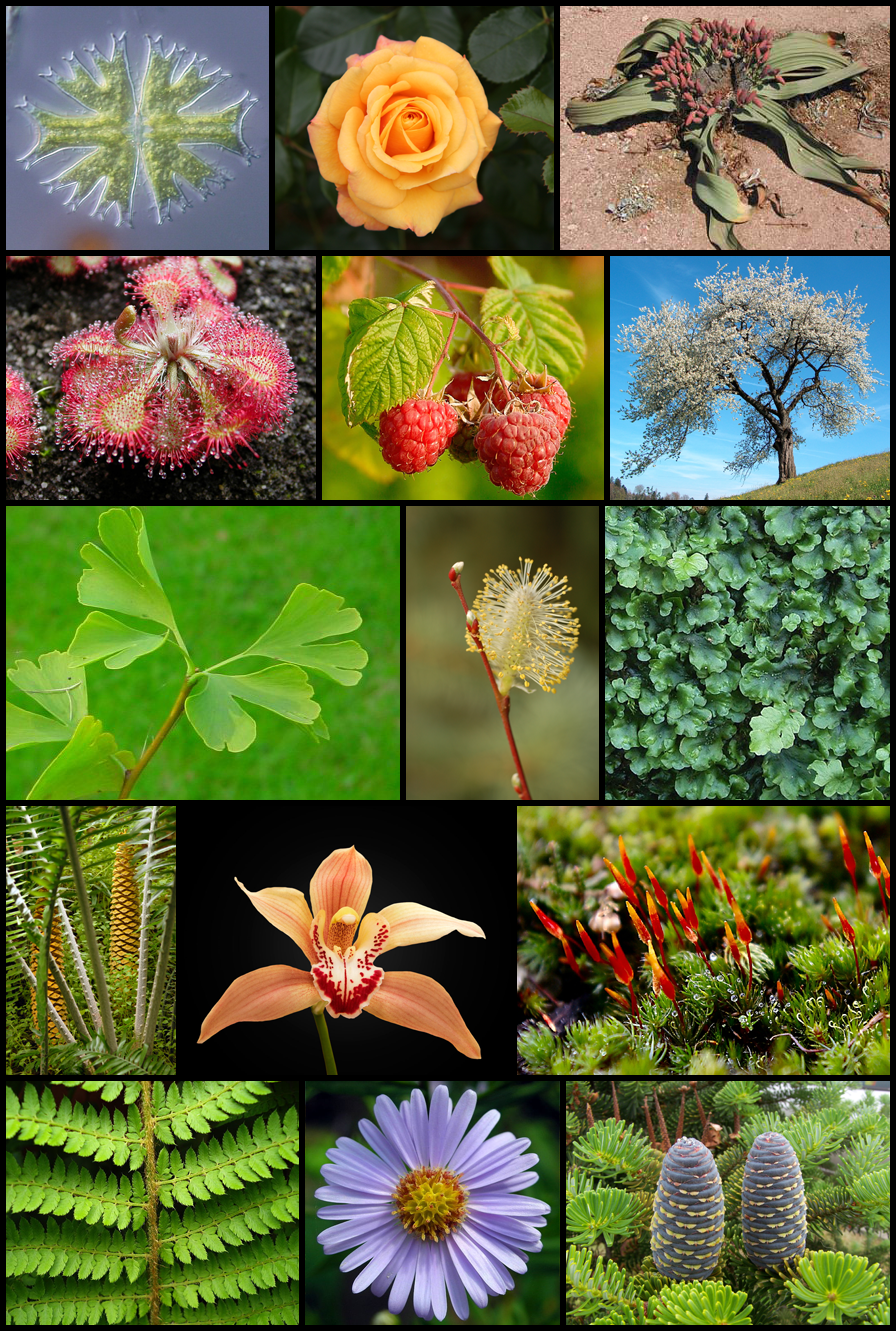
\includegraphics[width=0.7\linewidth]{./figures/plants/Diversity_of_plants_image_version_5} 

}

\caption{\href{https://commons.wikimedia.org/wiki/File:Diversity_of_plants_image_version_5.png}{The diversity of plants.}}\label{fig:plantdiversity}
\end{figure}

Green plants obtain most of their energy from sunlight via photosynthesis by primary chloroplasts that are derived from endosymbiosis with cyanobacteria. Their chloroplasts contain chlorophylls a and b, which gives them their green color. Some plants are parasitic or mycotrophic and have lost the ability to produce normal amounts of chlorophyll or to photosynthesize. Plants are characterized by sexual reproduction and alternation of generations, although asexual reproduction is also common.

There are about 320,000 species of plants, of which the great majority, some 260--290 thousand, produce seeds. Green plants provide a substantial proportion of the world's molecular oxygen, and are the basis of most of Earth's ecosystems. Plants that produce grain, fruit and vegetables also form basic human foods and have been domesticated for millennia. Plants have many cultural and other uses, as ornaments, building materials, writing material and, in great variety, they have been the source of medicines and psychoactive drugs. The scientific study of plants is known as botany, a branch of biology.

All living things were traditionally placed into one of two groups, plants and animals. This classification may date from Aristotle (384 BC -- 322 BC), who made the distinction between plants, which generally do not move, and animals, which often are mobile to catch their food. Much later, when Linnaeus (1707--1778) created the basis of the modern system of scientific classification, these two groups became the kingdoms Vegetabilia (later Metaphyta or Plantae) and Animalia (also called Metazoa). Since then, it has become clear that the plant kingdom as originally defined included several unrelated groups, and the fungi and several groups of algae were removed to new kingdoms. However, these organisms are still often considered plants, particularly in popular contexts.

The term ``plant'' generally implies the possession of the following traits: multicellularity, possession of cell walls containing cellulose, and the ability to carry out photosynthesis with primary chloroplasts.

When the name Plantae or plant is applied to a specific group of organisms or taxon, it usually refers to one of four concepts. From least to most inclusive, these four groupings are:

\onecolumn

\begin{sidewaystable}

\caption{\label{tab:plants}Four commonly used concepts of plants.}
\centering
\begin{tabular}[t]{>{\raggedright\arraybackslash}p{20em}>{\raggedright\arraybackslash}p{20em}>{\raggedright\arraybackslash}p{25em}}
\toprule
Name & Scope & Distribution\\
\midrule
\rowcolor{gray!6} Land plants (Embryophyta) & Plantae sensu strictissimo & Plants in the strictest sense include the liverworts, hornworts, mosses, and vascular plants, as well as fossil plants similar to these surviving groups.\\
Green plants (Viridiplantae or Viridiphyta or Chlorobionta or Chloroplastida) & Plantae sensu stricto & Plants in a strict sense include the green algae, and land plants that emerged within them, including stoneworts. The relationships between plant groups are still being worked out, and the names given to them vary considerably. The clade Viridiplantae encompasses a group of organisms that have cellulose in their cell walls, possess chlorophylls a and b and have plastids bound by only two membranes that are capable of photosynthesis and of storing starch. This clade is the main subject of this article.\\
\rowcolor{gray!6} Archaeplastida (Plastida or Primoplantae) & Plantae sensu lato & Plants in a broad sense comprise the green plants listed above plus the red algae (Rhodophyta) and the glaucophyte algae (Glaucophyta) that store Floridean starch outside the plastids, in the cytoplasm. This clade includes all of the organisms that eons ago acquired their primary chloroplasts directly by engulfing cyanobacteria.\\
Old definitions of plant (obsolete) & Plantae sensu amplo & Plants in the widest sense refers to older, obsolete classifications that placed diverse algae, fungi or bacteria in Plantae .\\
\bottomrule
\end{tabular}
\end{sidewaystable}

\twocolumn

The evolution of plants has resulted in increasing levels of complexity, from the earliest algal mats, through bryophytes, lycopods, ferns to the complex gymnosperms and angiosperms of today. Plants in all of these groups continue to thrive, especially in the environments in which they evolved.

An algal scum formed on the land 1,200 million years ago, but it was not until the Ordovician Period, around 450 million years ago, that land plants appeared. However, new evidence from the study of carbon isotope ratios in Precambrian rocks has suggested that complex photosynthetic plants developed on the earth over 1000 m.y.a. For more than a century it has been assumed that the ancestors of land plants evolved in aquatic environments and then adapted to a life on land, an idea usually credited to botanist Frederick Orpen Bower in his 1908 book The Origin of a Land Flora. A recent alternative view, supported by genetic evidence, is that they evolved from terrestrial single-celled algae, and that even the common ancestor of red and green algae, and the unicellular freshwater algae glaucophytes, originated in a terrestrial environment in freshwater biofilms or microbial mats. Primitive land plants began to diversify in the late Silurian Period, around 420 million years ago, and the results of their diversification are displayed in remarkable detail in an early Devonian fossil assemblage from the Rhynie chert. This chert preserved early plants in cellular detail, petrified in volcanic springs. By the middle of the Devonian Period most of the features recognised in plants today are present, including roots, leaves and secondary wood, and by late Devonian times seeds had evolved. Late Devonian plants had thereby reached a degree of sophistication that allowed them to form forests of tall trees. Evolutionary innovation continued in the Carboniferous and later geological periods and is ongoing today. Most plant groups were relatively unscathed by the Permo-Triassic extinction event, although the structures of communities changed. This may have set the scene for the evolution of flowering plants in the Triassic (\textasciitilde200 million years ago), which exploded in the Cretaceous and Tertiary. The latest major group of plants to evolve were the grasses, which became important in the mid Tertiary, from around 40 million years ago. The grasses, as well as many other groups, evolved new mechanisms of metabolism to survive the low CO\textsubscript{2} and warm, dry conditions of the tropics over the last 10 million years.

\hypertarget{embryophytes}{%
\section{Embryophytes}\label{embryophytes}}

The plants that are likely most familiar to us are the multicellular land plants, called embryophytes. Embryophytes include the vascular plants, such as ferns, conifers and flowering plants. They also include the bryophytes, of which mosses and liverworts are the most common.

All of these plants have eukaryotic cells with cell walls composed of cellulose, and most obtain their energy through photosynthesis, using light, water and carbon dioxide to synthesize food. About three hundred plant species do not photosynthesize but are parasites on other species of photosynthetic plants. Embryophytes are distinguished from green algae, which represent a mode of photosynthetic life similar to the kind modern plants are believed to have evolved from, by having specialized reproductive organs protected by non-reproductive tissues.

Bryophytes first appeared during the early Paleozoic. They mainly live in habitats where moisture is available for significant periods, although some species, such as Targionia, are desiccation-tolerant. Most species of bryophytes remain small throughout their life-cycle. This involves an alternation between two generations: a haploid stage, called the gametophyte, and a diploid stage, called the sporophyte. In bryophytes, the sporophyte is always unbranched and remains nutritionally dependent on its parent gametophyte. The embryophytes have the ability to secrete a cuticle on their outer surface, a waxy layer that confers resistant to desiccation. In the mosses and hornworts a cuticle is usually only produced on the sporophyte. Stomata are absent from liverworts, but occur on the sporangia of mosses and hornworts, allowing gas exchange.

Vascular plants first appeared during the Silurian period, and by the Devonian had diversified and spread into many different terrestrial environments. They developed a number of adaptations that allowed them to spread into increasingly more arid places, notably the vascular tissues xylem and phloem, that transport water and food throughout the organism. Root systems capable of obtaining soil water and nutrients also evolved during the Devonian. In modern vascular plants, the sporophyte is typically large, branched, nutritionally independent and long-lived, but there is increasing evidence that Paleozoic gametophytes were just as complex as the sporophytes. The gametophytes of all vascular plant groups evolved to become reduced in size and prominence in the life cycle.

In seed plants, the microgametophyte is reduced from a multicellular free-living organism to a few cells in a pollen grain and the miniaturised megagametophyte remains inside the megasporangium, attached to and dependent on the parent plant. A megasporangium enclosed in a protective layer called an integument is known as an ovule. After fertilisation by means of sperm produced by pollen grains, an embryo sporophyte develops inside the ovule. The integument becomes a seed coat, and the ovule develops into a seed. Seed plants can survive and reproduce in extremely arid conditions, because they are not dependent on free water for the movement of sperm, or the development of free living gametophytes.

The first seed plants, pteridosperms (seed ferns), now extinct, appeared in the Devonian and diversified through the Carboniferous. They were the ancestors of modern gymnosperms, of which four surviving groups are widespread today, particularly the conifers, which are dominant trees in several biomes. The name gymnosperm comes from the Greek composite word γυμνόσπερμος (γυμνός gymnos, ``naked'' and σπέρμα sperma, ``seed''), as the ovules and subsequent seeds are not enclosed in a protective structure (carpels or fruit), but are borne naked, typically on cone scales.

Plant fossils include roots, wood, leaves, seeds, fruit, pollen, spores, phytoliths, and amber (the fossilized resin produced by some plants). Fossil land plants are recorded in terrestrial, lacustrine, fluvial and nearshore marine sediments. Pollen, spores and algae (dinoflagellates and acritarchs) are used for dating sedimentary rock sequences. The remains of fossil plants are not as common as fossil animals, although plant fossils are locally abundant in many regions worldwide.

The earliest fossils clearly assignable to Kingdom Plantae are fossil green algae from the Cambrian. These fossils resemble calcified multicellular members of the Dasycladales. Earlier Precambrian fossils are known that resemble single-cell green algae, but definitive identity with that group of algae is uncertain.

The earliest fossils attributed to green algae date from the Precambrian (ca. 1200 mya). The resistant outer walls of prasinophyte cysts (known as phycomata) are well preserved in fossil deposits of the Paleozoic (ca. 250--540 mya). A filamentous fossil (Proterocladus) from middle Neoproterozoic deposits (ca. 750 mya) has been attributed to the Cladophorales, while the oldest reliable records of the Bryopsidales, Dasycladales) and stoneworts are from the Paleozoic.

The oldest known fossils of embryophytes date from the Ordovician, though such fossils are fragmentary. By the Silurian, fossils of whole plants are preserved, including the simple vascular plant Cooksonia in mid-Silurian and the much larger and more complex lycophyte Baragwanathia longifolia in late Silurian. From the early Devonian Rhynie chert, detailed fossils of lycophytes and rhyniophytes have been found that show details of the individual cells within the plant organs and the symbiotic association of these plants with fungi of the order Glomales. The Devonian period also saw the evolution of leaves and roots, and the first modern tree, Archaeopteris. This tree with fern-like foliage and a trunk with conifer-like wood was heterosporous producing spores of two different sizes, an early step in the evolution of seeds.



\begin{figure}

{\centering 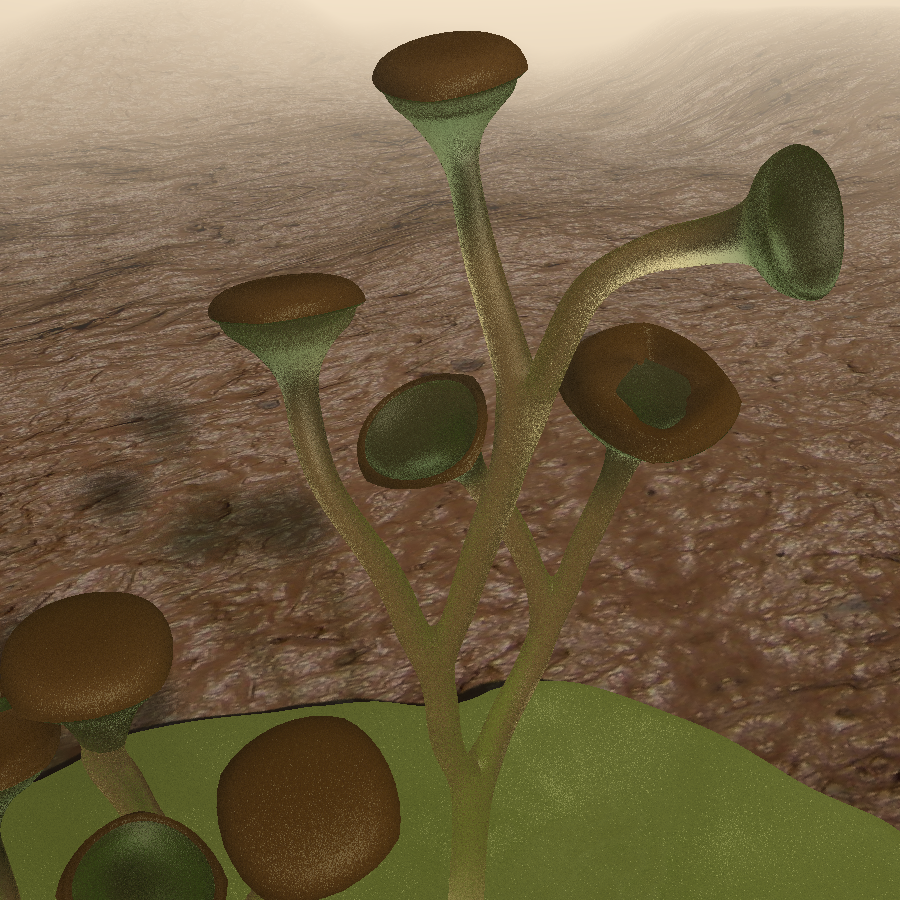
\includegraphics[width=0.7\linewidth]{./figures/plants/Cooksonia_pertoni} 

}

\caption{\href{https://commons.wikimedia.org/wiki/File:Cooksonia_pertoni.png}{Reconstruction of Cooksonia, a vascular plant from the Silurian}}\label{fig:cooksonia}
\end{figure}

The Coal measures are a major source of Paleozoic plant fossils, with many groups of plants in existence at this time. The spoil heaps of coal mines are the best places to collect; coal itself is the remains of fossilised plants, though structural detail of the plant fossils is rarely visible in coal. In the Fossil Grove at Victoria Park in Glasgow, Scotland, the stumps of Lepidodendron trees are found in their original growth positions.

The fossilized remains of conifer and angiosperm roots, stems and branches may be locally abundant in lake and inshore sedimentary rocks from the Mesozoic and Cenozoic eras. Sequoia and its allies, magnolia, oak, and palms are often found.

Petrified wood is common in some parts of the world, and is most frequently found in arid or desert areas where it is more readily exposed by erosion. Petrified wood is often heavily silicified (the organic material replaced by silicon dioxide), and the impregnated tissue is often preserved in fine detail. Such specimens may be cut and polished using lapidary equipment. Fossil forests of petrified wood have been found in all continents.

Fossils of seed ferns such as Glossopteris are widely distributed throughout several continents of the Southern Hemisphere, a fact that gave support to Alfred Wegener's early ideas regarding Continental drift theory.

\hypertarget{non-vascular-plants}{%
\section{Non-vascular Plants}\label{non-vascular-plants}}

Bryophytes are an informal group consisting of three divisions of non-vascular land plants (embryophytes): the liverworts, hornworts and mosses. They are characteristically limited in size and prefer moist habitats although they can survive in drier environments. The bryophytes consist of about 20,000 plant species. Bryophytes produce enclosed reproductive structures (gametangia and sporangia), but they do not produce flowers or seeds. They reproduce via spores. Bryophytes are usually considered to be a paraphyletic group and not a monophyletic group, although some studies have produced contrary results. Regardless of their status, the name is convenient and remains in use as an informal collective term. The term ``bryophyte'' comes from Greek βρύον, bryon ``tree-moss, oyster-green'' and φυτόν, phyton ``plant''.



\begin{figure}

{\centering 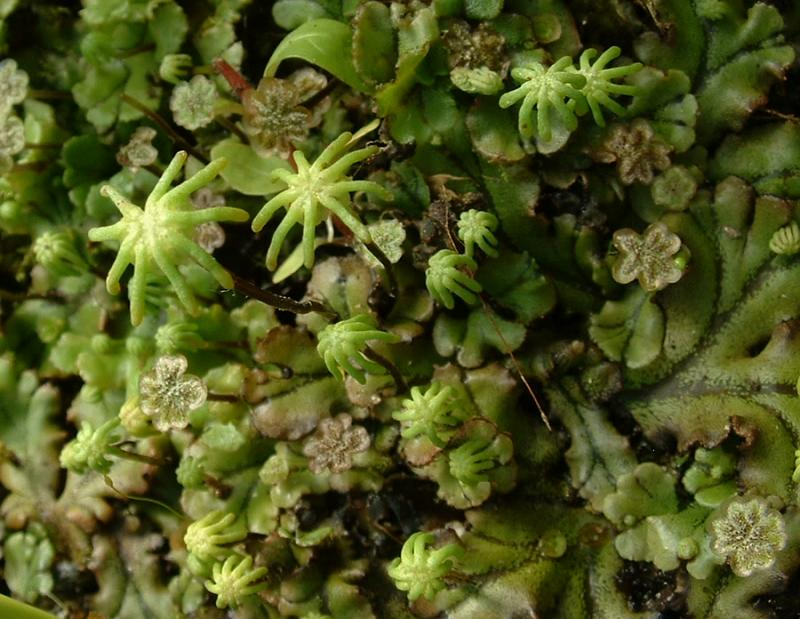
\includegraphics[width=0.7\linewidth]{./figures/plants/Marchantia} 

}

\caption{\href{https://upload.wikimedia.org/wikipedia/commons/d/dc/Marchantia.jpg}{Marchantia polymorpha, with antheridial and archegonial stalks.}}\label{fig:marchantia}
\end{figure}



\begin{figure}

{\centering 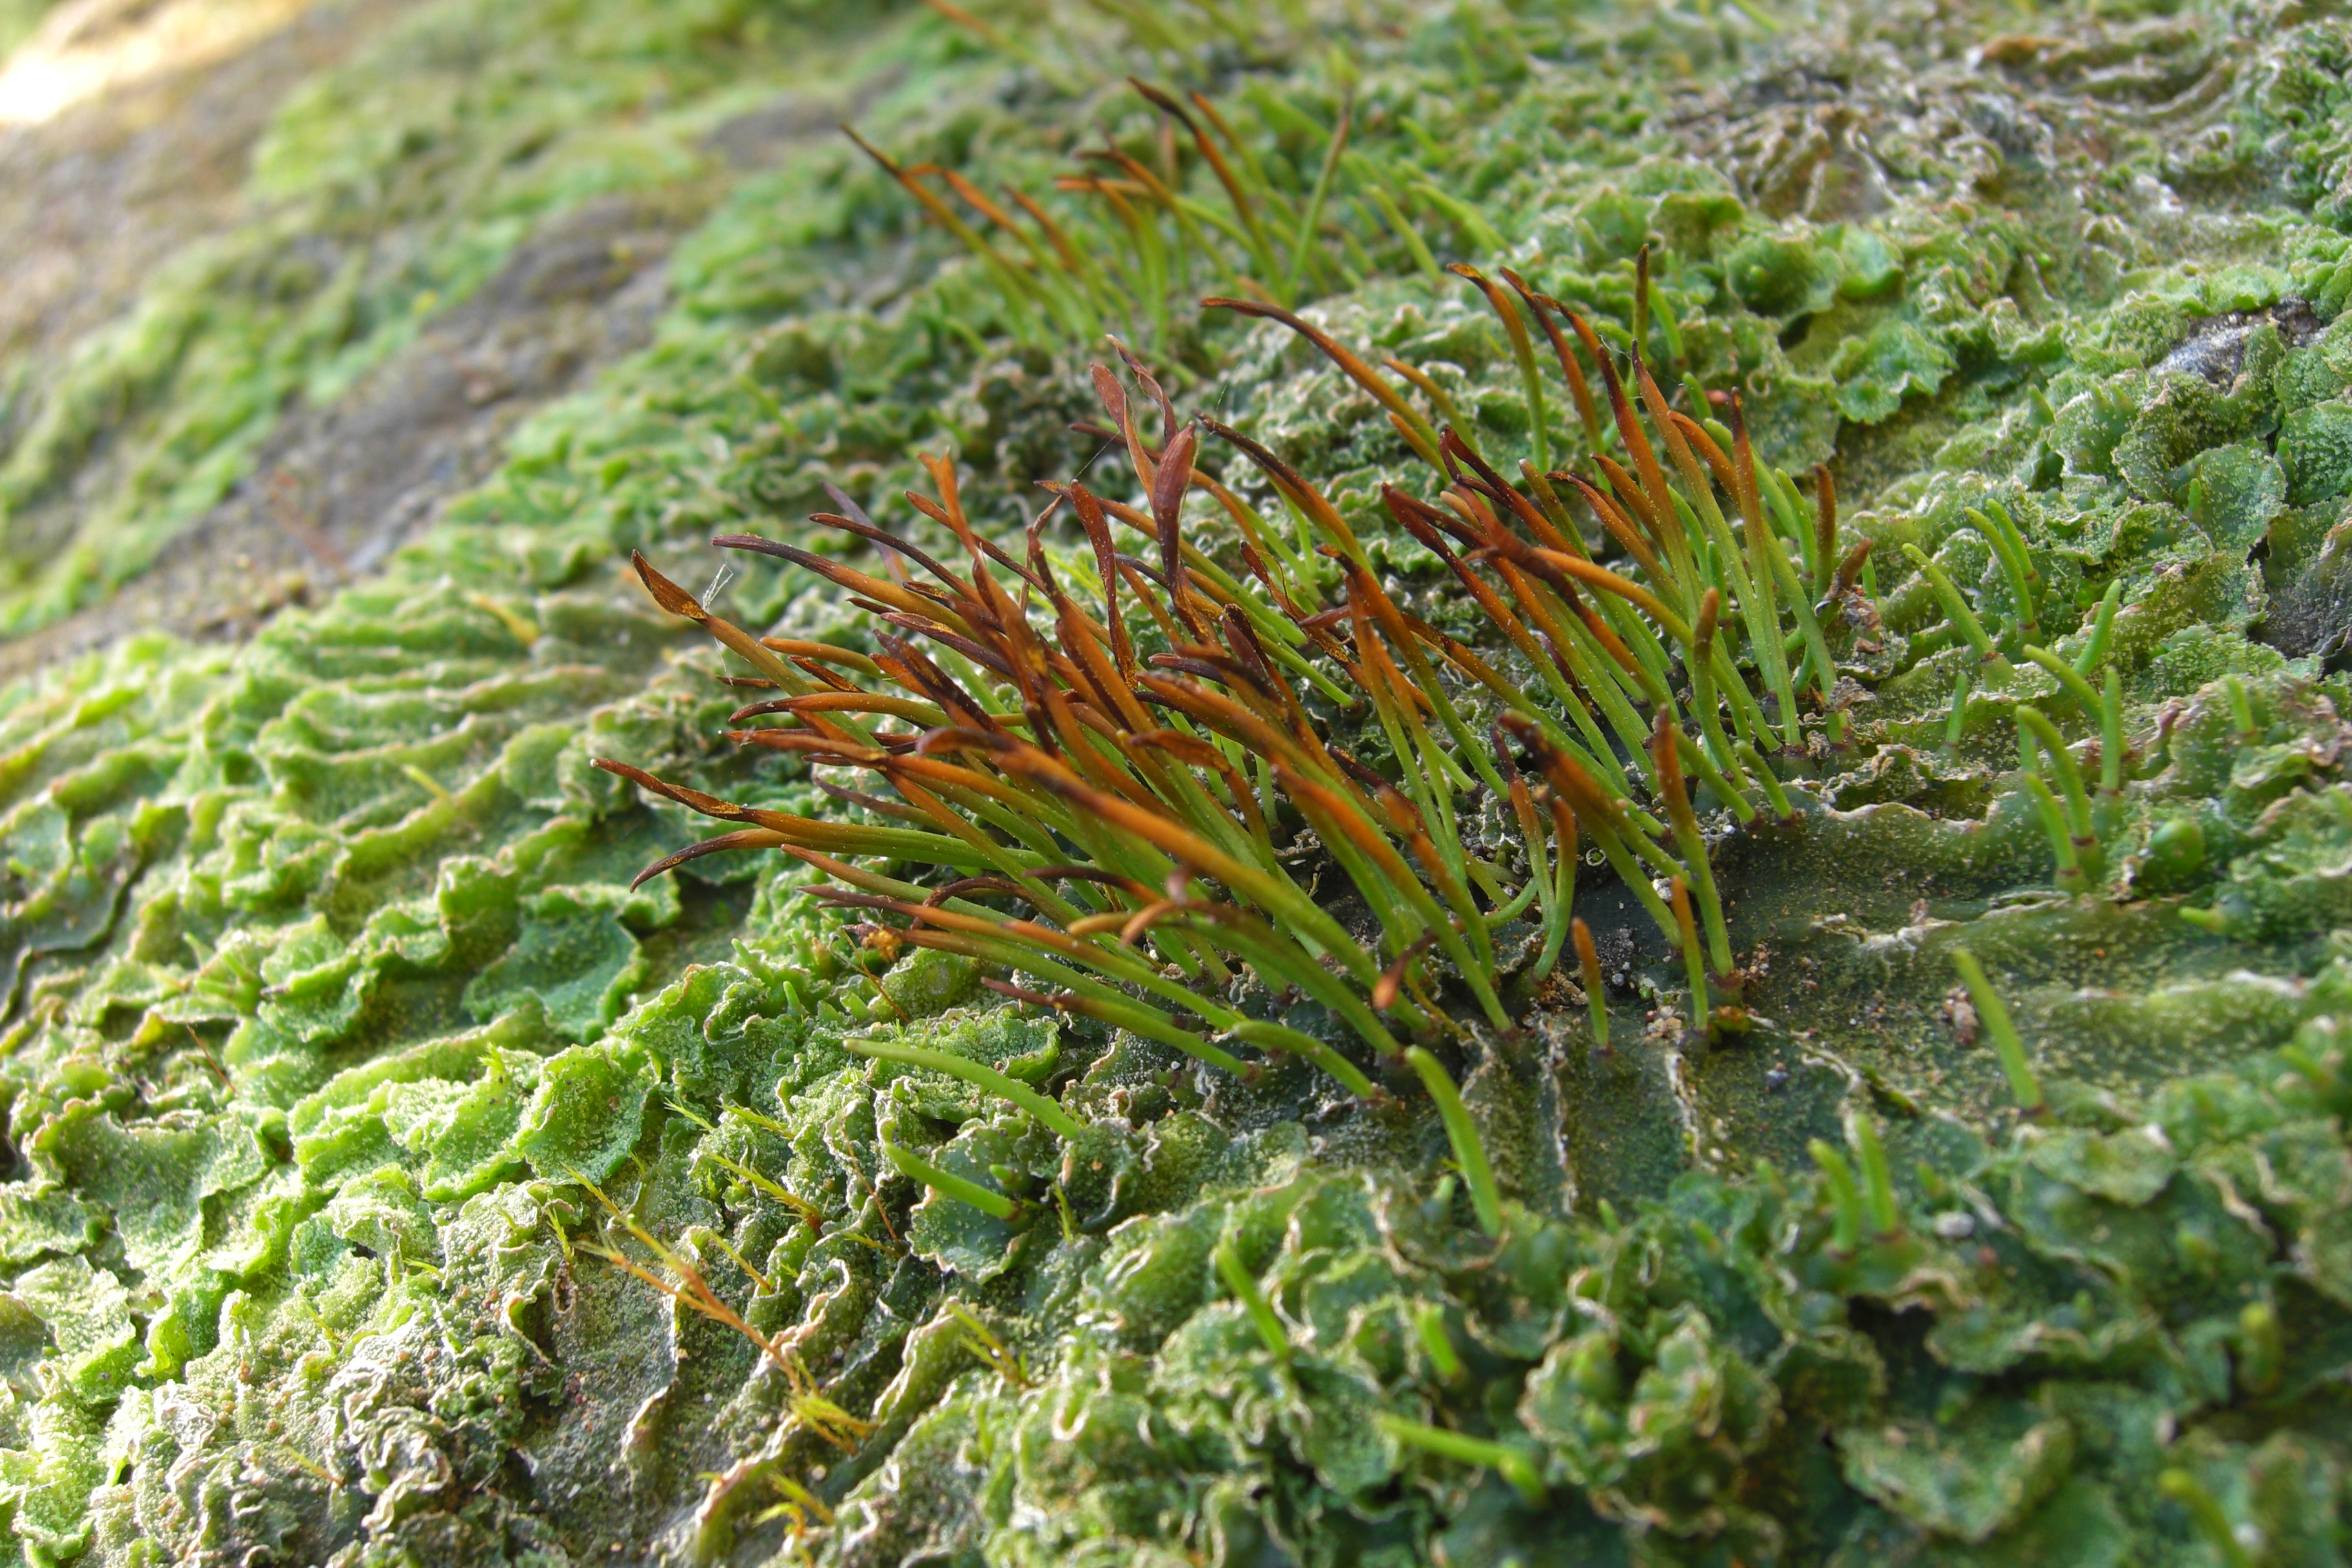
\includegraphics[width=0.7\linewidth]{./figures/plants/Hornwort_(3144429129)} 

}

\caption{\href{https://commons.wikimedia.org/wiki/File:Hornwort_(3144429129).jpg}{Hornworts are bryophytes that are believed to the closest living relatives of the vascular plants.}}\label{fig:hornwort}
\end{figure}



\begin{figure}

{\centering 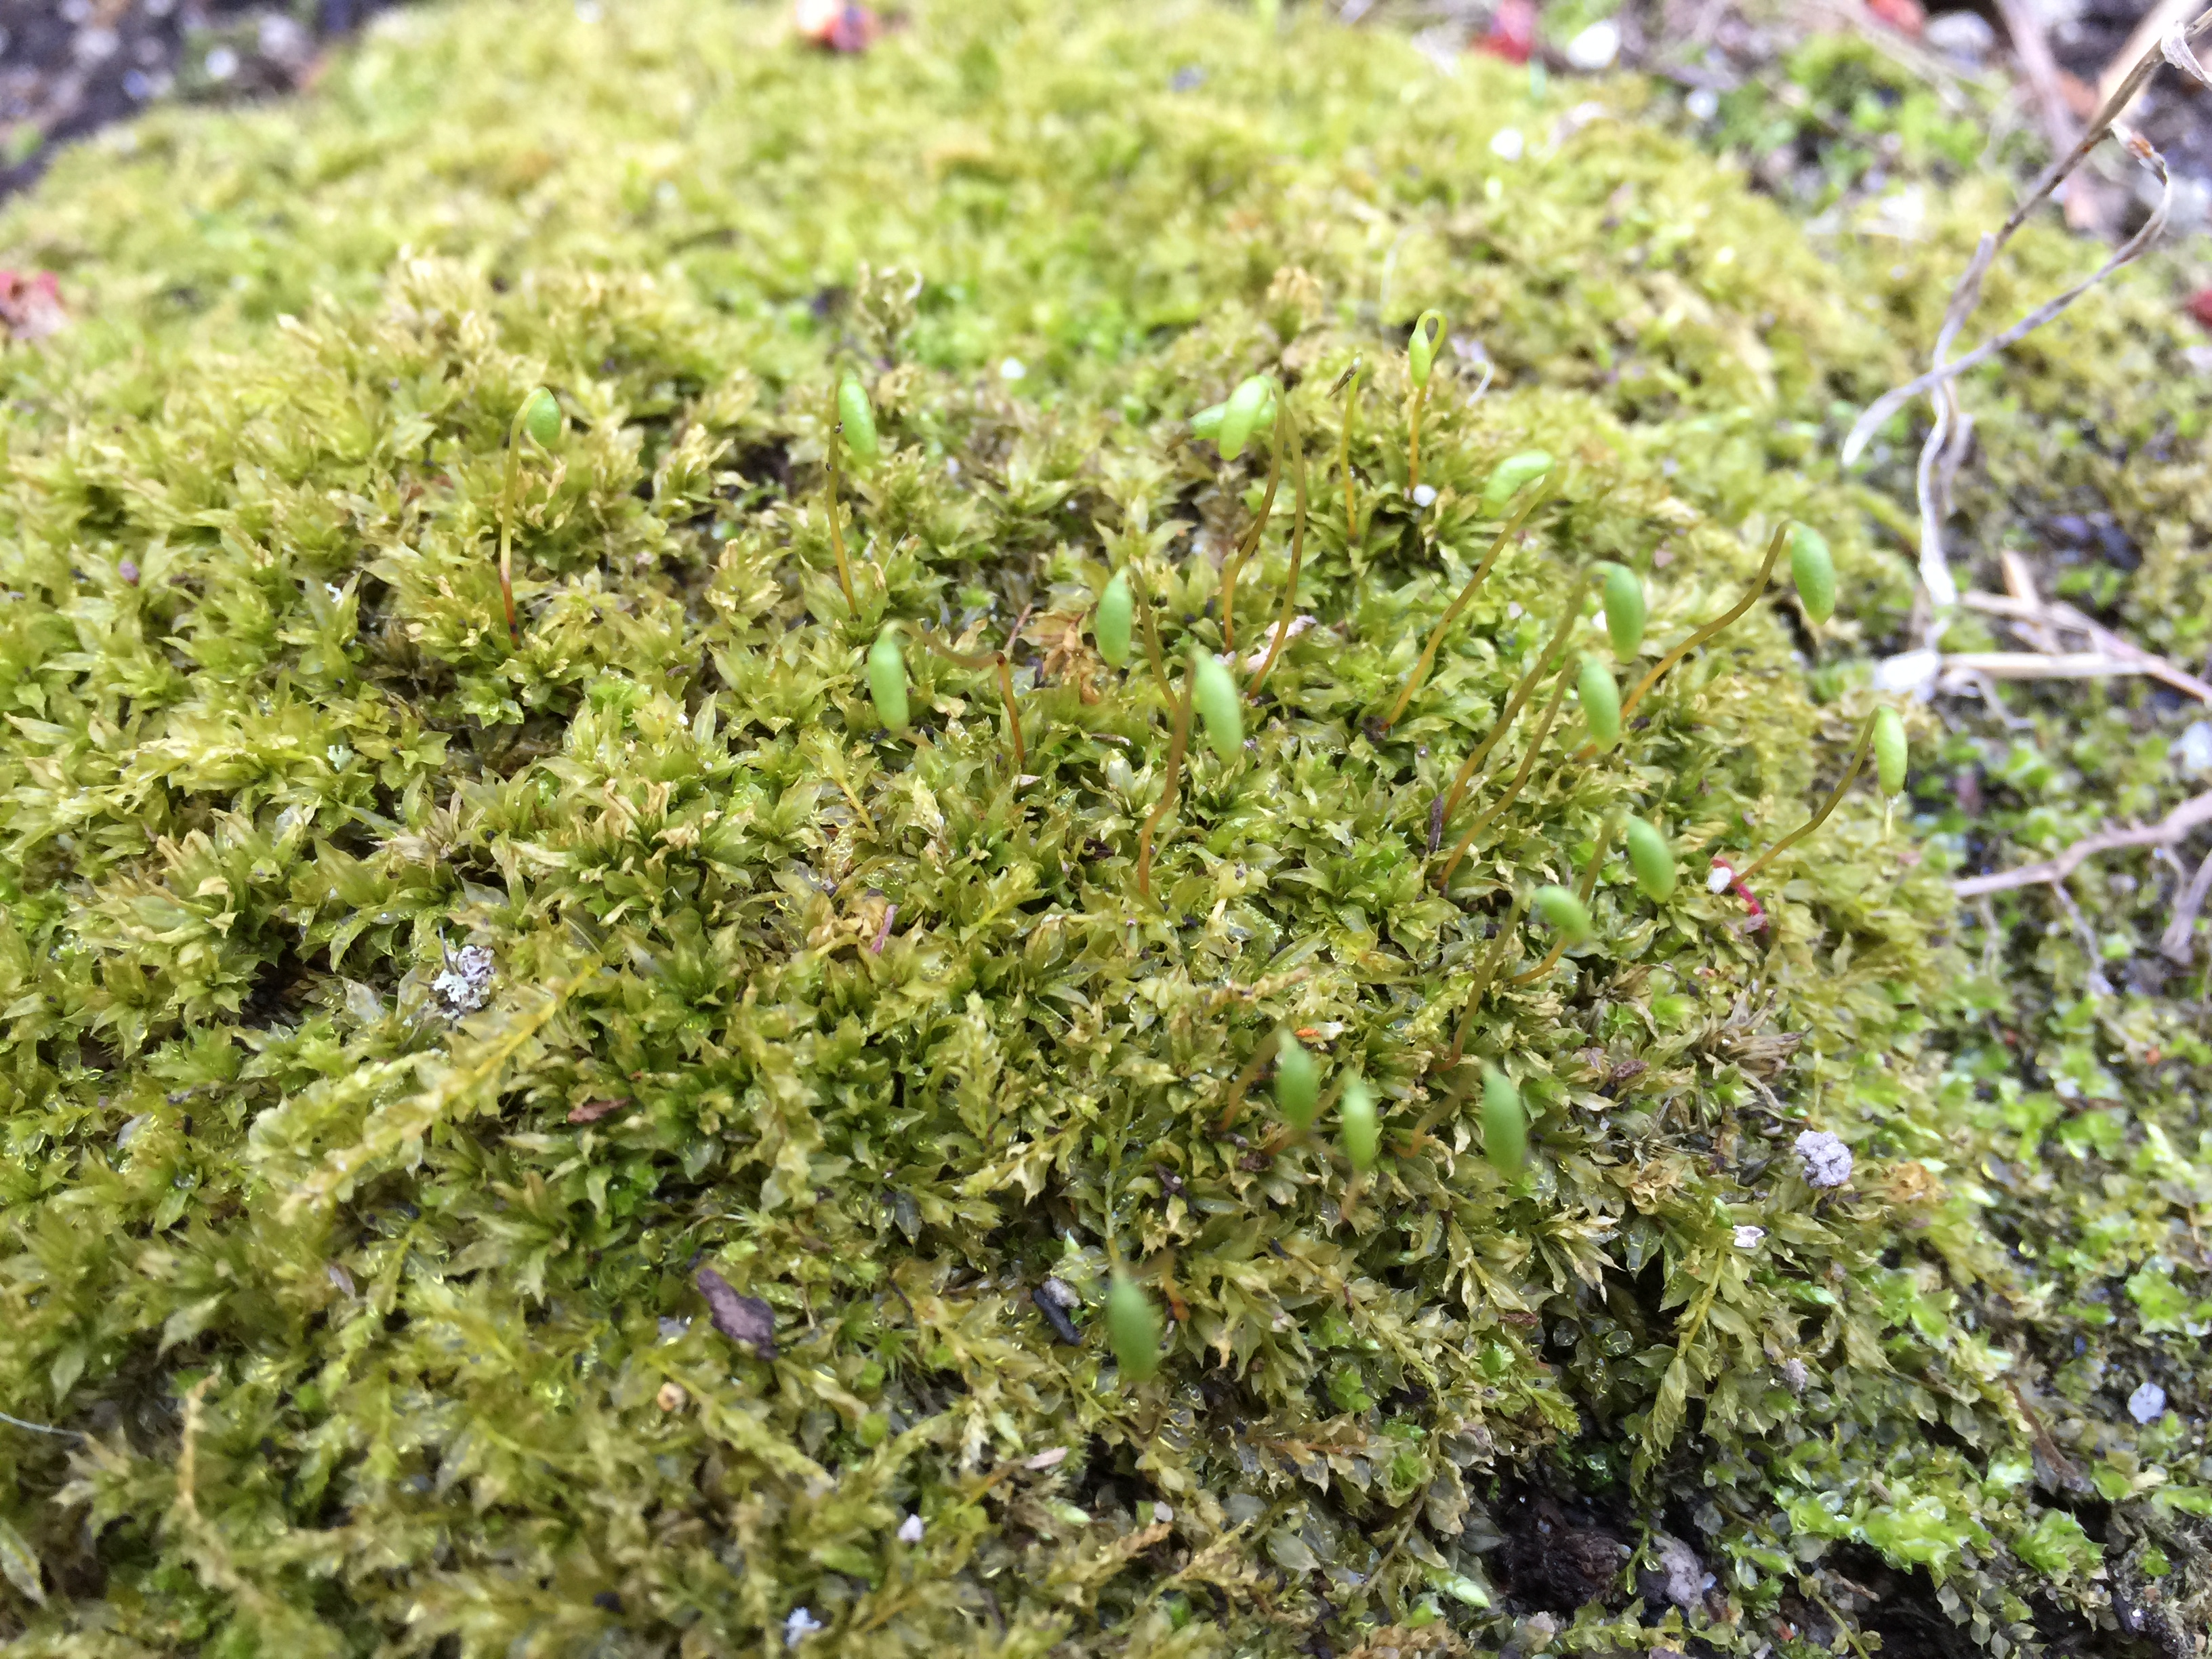
\includegraphics[width=0.7\linewidth]{./figures/plants/IMG_1227} 

}

\caption{A moss showing both gametophytes (the low, leaf-like forms) and sporophytes (the tall, stalk-like forms).}\label{fig:sporophytemoss}
\end{figure}

The defining features of bryophytes are:

\begin{itemize}
\tightlist
\item
  Their life cycles are dominated by the gametophyte stage
\item
  Their sporophytes are unbranched
\item
  They do not have a true vascular tissue containing lignin (although some have specialized tissues for the transport of water)
\end{itemize}

Bryophytes exist in a wide variety of habitats. They can be found growing in a range of temperatures (cold arctics and in hot deserts), elevations (sea-level to alpine), and moisture (dry deserts to wet rainforests).

Bryophytes can grow where vascularized plants cannot because they do not depend on roots for an uptake of nutrients from soil. Bryophytes can survive on rocks and bare soil.

Traditionally, all living land plants without vascular tissues were classified in a single taxonomic group, often a division (or phylum). More recently, phylogenetic research has questioned whether the bryophytes form a monophyletic group and thus whether they should form a single taxon. Although a 2005 study supported the traditional view that the bryophytes form a monophyletic group, by 2010 a broad consensus had emerged among systematists that bryophytes as a whole are not a natural group (i.e., are paraphyletic), although each of the three extant (living) groups is monophyletic.

The three bryophyte clades (which may be treated as divisions) are the Marchantiophyta (liverworts), Bryophyta (mosses) and Anthocerotophyta (hornworts). The vascular plants or tracheophytes form a fourth, unranked clade of land plants called the ``Polysporangiophyta''. In this analysis, hornworts are sister to vascular plants and liverworts are sister to all other land plants, including the hornworts and mosses. Phylogenetic studies continue to produce conflicting results. In particular those based on gene sequences suggest the bryophytes are paraphyletic, whereas those based on the amino acid translations of the same genes suggest they are monophyletic. A 2014 study concluded that composition biases were responsible for these differences and that the bryophytes are monophyletic. The issue remains unresolved.

\hypertarget{vascular-plants}{%
\section{Vascular Plants}\label{vascular-plants}}

Vascular plants (from Latin vasculum: duct), also known as tracheophytes (from the equivalent Greek term trachea), form a large group of plants (c.~308,312 accepted known species) that are defined as land plants that have lignified tissues (the xylem) for conducting water and minerals throughout the plant. They also have a specialized non-lignified tissue (the phloem) to conduct products of photosynthesis. Vascular plants include the clubmosses, horsetails, ferns, gymnosperms (including conifers) and angiosperms (flowering plants). Scientific names for the group include Tracheophyta,:251 Tracheobionta and Equisetopsida sensu lato. Some early land plants (the rhyniophytes) had less developed vascular tissue; the term eutracheophyte has been used for all other vascular plants.

Botanists define vascular plants by three primary characteristics:

\begin{itemize}
\tightlist
\item
  Vascular plants have vascular tissues which distribute resources through the plant. Two kinds of vascular tissue occur in plants: xylem and phloem. Phloem and xylem are closely associated with one another and are typically located immediately adjacent to each other in the plant. The combination of one xylem and one phloem strand adjacent to each other is known as a vascular bundle. The evolution of vascular tissue in plants allowed them to evolve to larger sizes than non-vascular plants, which lack these specialized conducting tissues and are thereby restricted to relatively small sizes.
\item
  In vascular plants, the principal generation phase is the sporophyte, which produces spores and is diploid (having two sets of chromosomes per cell). (By contrast, the principal generation phase in non-vascular plants is the gametophyte, which produces gametes and is haploid - with one set of chromosomes per cell.)
\item
  Vascular plants have true roots, leaves, and stems, even if some groups have secondarily lost one or more of these traits.
\end{itemize}

Cavalier-Smith (1998) treated the Tracheophyta as a phylum or botanical division encompassing two of these characteristics defined by the Latin phrase ``facies diploida xylem et phloem instructa'' (diploid phase with xylem and phloem).:251

One possible mechanism for the presumed evolution from emphasis on haploid generation to emphasis on diploid generation is the greater efficiency in spore dispersal with more complex diploid structures. Elaboration of the spore stalk enabled the production of more spores and the development of the ability to release them higher and to broadcast them farther. Such developments may include more photosynthetic area for the spore-bearing structure, the ability to grow independent roots, woody structure for support, and more branching.

Water and nutrients in the form of inorganic solutes are drawn up from the soil by the roots and transported throughout the plant by the xylem. Organic compounds such as sucrose produced by photosynthesis in leaves are distributed by the phloem sieve tube elements.

The xylem consists of vessels in flowering plants and tracheids in other vascular plants, which are dead hard-walled hollow cells arranged to form files of tubes that function in water transport. A tracheid cell wall usually contains the polymer lignin. The phloem, however, consists of living cells called sieve-tube members. Between the sieve-tube members are sieve plates, which have pores to allow molecules to pass through. Sieve-tube members lack such organs as nuclei or ribosomes, but cells next to them, the companion cells, function to keep the sieve-tube members alive.

The most abundant compound in all plants, as in all cellular organisms, is water, which serves an important structural role and a vital role in plant metabolism. Transpiration is the main process of water movement within plant tissues. Water is constantly transpired from the plant through its stomata to the atmosphere and replaced by soil water taken up by the roots. The movement of water out of the leaf stomata creates a transpiration pull or tension in the water column in the xylem vessels or tracheids. The pull is the result of water surface tension within the cell walls of the mesophyll cells, from the surfaces of which evaporation takes place when the stomata are open. Hydrogen bonds exist between water molecules, causing them to line up; as the molecules at the top of the plant evaporate, each pulls the next one up to replace it, which in turn pulls on the next one in line. The draw of water upwards may be entirely passive and can be assisted by the movement of water into the roots via osmosis. Consequently, transpiration requires very little energy to be used by the plant. Transpiration assists the plant in absorbing nutrients from the soil as soluble salts.

Living root cells passively absorb water in the absence of transpiration pull via osmosis creating root pressure. It is possible for there to be no evapotranspiration and therefore no pull of water towards the shoots and leaves. This is usually due to high temperatures, high humidity, darkness or drought.

Xylem and phloem tissues are involved in the conduction processes within plants. Sugars are conducted throughout the plant in the phloem, water and other nutrients through the xylem. Conduction occurs from a source to a sink for each separate nutrient. Sugars are produced in the leaves (a source) by photosynthesis and transported to the growing shoots and roots (sinks) for use in growth, cellular respiration or storage. Minerals are absorbed in the roots (a source) and transported to the shoots to allow cell division and growth.

\hypertarget{ferns}{%
\subsection{Ferns}\label{ferns}}

A fern (Polypodiopsida or Polypodiophyta) is a member of a group of vascular plants (plants with xylem and phloem) that reproduce via spores and have neither seeds nor flowers. They differ from mosses by being vascular, i.e., having specialized tissues that conduct water and nutrients and in having life cycles in which the sporophyte is the dominant phase. Ferns have complex leaves called megaphylls, that are more complex than the microphylls of clubmosses. Most ferns are leptosporangiate ferns. They produce coiled fiddleheads that uncoil and expand into fronds. The group includes about 10,560 known extant species. Ferns are defined here in the broad sense, being all of the Polypodiopsida, comprising both the leptosporangiate (Polypodiidae) and eusporangiate ferns, the latter group including horsetails or scouring rushes, whisk ferns, marattioid ferns, and ophioglossoid ferns.

Ferns first appear in the fossil record about 360 million years ago in the middle Devonian period, but many of the current families and species did not appear until roughly 145 million years ago in the early Cretaceous, after flowering plants came to dominate many environments. The fern Osmunda claytoniana is a paramount example of evolutionary stasis; paleontological evidence indicates it has remained unchanged, even at the level of fossilized nuclei and chromosomes, for at least 180 million years.

Ferns are not of major economic importance, but some are used for food, medicine, as biofertilizer, as ornamental plants and for remediating contaminated soil. They have been the subject of research for their ability to remove some chemical pollutants from the atmosphere. Some fern species, such as bracken (Pteridium aquilinum) and water fern (Azolla filiculoides) are significant weeds worldwide. Some fern genera, such as Azolla, can fix nitrogen and make a significant input to the nitrogen nutrition of rice paddies. They also play certain roles in folklore.

Like the sporophytes of seed plants, those of ferns consist of stems, leaves and roots. Ferns differ from seed plants in reproducing by spores and from bryophytes in that, like seed plants, they are Polysporangiophytes, their sporophytes branching and producing many sporangia. Unlike bryophytes, fern sporophytes are free-living and only briefly dependent on the maternal gametophyte.

Stems: Fern stems are often referred to as rhizomes, even though they grow underground only in some of the species. Epiphytic species and many of the terrestrial ones have above-ground creeping stolons (e.g., Polypodiaceae), and many groups have above-ground erect semi-woody trunks (e.g., Cyatheaceae). These can reach up to 20 meters (66 ft) tall in a few species (e.g., Cyathea brownii on Norfolk Island and Cyathea medullaris in New Zealand).

Leaf: The green, photosynthetic part of the plant is technically a megaphyll and in ferns, it is often referred to as a frond. New leaves typically expand by the unrolling of a tight spiral called a crozier or fiddlehead into fronds. This uncurling of the leaf is termed circinate vernation. Leaves are divided into two types a trophophyll and a sporophyll. A trophophyll frond is a vegetative leaf analogous to the typical green leaves of seed plants that does not produce spores, instead only producing sugars by photosynthesis. A sporophyll frond is a fertile leaf that produces spores borne in sporangia that are usually clustered to form sori. In most ferns, fertile leaves are morphologically very similar to the sterile ones, and they photosynthesize in the same way. In some groups, the fertile leaves are much narrower than the sterile leaves, and may even have no green tissue at all (e.g., Blechnaceae, Lomariopsidaceae). The anatomy of fern leaves can either be simple or highly divided. In tree ferns, the main stalk that connects the leaf to the stem (known as the stipe), often has multiple leaflets. The leafy structures that grow from the stipe are known as pinnae and are often again divided into smaller pinnules.

Roots: The underground non-photosynthetic structures that take up water and nutrients from soil. They are always fibrous and structurally are very similar to the roots of seed plants.

Like all other vascular plants, the diploid sporophyte is the dominant phase or generation in the life cycle. The gametophytes of ferns, however, are very different from those of seed plants. They are free-living and resemble liverworts, whereas those of seed plants develop within the spore wall and are dependent on the parent sporophyte for their nutrition. A fern gametophyte typically consists of:

Prothallus: A green, photosynthetic structure that is one cell thick, usually heart or kidney shaped, 3--10 mm long and 2--8 mm broad. The prothallus produces gametes by means of:
Antheridia: Small spherical structures that produce flagellate sperm.
Archegonia: A flask-shaped structure that produces a single egg at the bottom, reached by the sperm by swimming down the neck.
Rhizoids: root-like structures (not true roots) that consist of single greatly elongated cells, that absorb water and mineral salts over the whole structure. Rhizoids anchor the prothallus to the soil.

Ferns are widespread in their distribution, with the greatest abundance in the tropics, and least in arctic areas. The greatest diversity occurs in tropical rainforests. New Zealand, for which the fern is a symbol, has about 230 species, distributed throughout the country.

The stereotypical image of ferns growing in moist shady woodland nooks is far from a complete picture of the habitats where ferns can be found growing. Fern species live in a wide variety of habitats, from remote mountain elevations, to dry desert rock faces, to bodies of water or in open fields. Ferns in general may be thought of as largely being specialists in marginal habitats, often succeeding in places where various environmental factors limit the success of flowering plants. Some ferns are among the world's most serious weed species, including the bracken fern growing in the Scottish highlands, or the mosquito fern (Azolla) growing in tropical lakes, both species forming large aggressively spreading colonies. There are four particular types of habitats that ferns are found in: moist, shady forests; crevices in rock faces, especially when sheltered from the full sun; acid wetlands including bogs and swamps; and tropical trees, where many species are epiphytes (something like a quarter to a third of all fern species).

Especially the epiphytic ferns have turned out to be hosts of a huge diversity of invertebrates. It is assumed that bird's-nest ferns alone contain up to half the invertebrate biomass within a hectare of rainforest canopy.

Many ferns depend on associations with mycorrhizal fungi. Many ferns grow only within specific pH ranges; for instance, the climbing fern (Lygodium palmatum) of eastern North America will grow only in moist, intensely acid soils, while the bulblet bladder fern (Cystopteris bulbifera), with an overlapping range, is found only on limestone.

The spores are rich in lipids, protein and calories, so some vertebrates eat these. The European woodmouse (Apodemus sylvaticus) has been found to eat the spores of Culcita macrocarpa and the bullfinch (Pyrrhula murina) and the New Zealand lesser short-tailed bat (Mystacina tuberculata) also eat fern spores.

\hypertarget{seed-plants}{%
\section{Seed Plants}\label{seed-plants}}

The spermatophytes, also known as phanerogams (taxon Phanerogamae) or phaenogams (taxon Phaenogamae), comprise those plants that produce seeds, hence the alternative name seed plants. They are a subset of the embryophytes or land plants. The term phanerogams or phanerogamae is derived from the Greek φανερός, phanerós meaning ``visible'', in contrast to the cryptogamae from Greek κρυπτός kryptós = ``hidden'' together with the suffix γαμέω, gameo, ``to marry''. These terms distinguished those plants with hidden sexual organs (cryptogamae) from those with visible sexual organs (phanerogamae).



\begin{figure}

{\centering \includegraphics[width=0.7\linewidth]{./figures/plants/seeds_diversity} 

}

\caption{\href{https://commons.wikimedia.org/wiki/File:Разнообразие_семян.jpg}{Microimages of seeds of various plants.} The first row: Poppy, Red pepper, Strawberry, Apple tree, Blackberry, Rice, Carum. Second row: Mustard, Eggplant, Physalis, grapes, raspberries, red rice, Patchouli. The third row: Figs, Lycium barbarum, Beets, Blueberries, Golden Kiwifruit, Rosehip, Basil. The fourth row: Pink pepper, Tomato, Radish, Carrot, Matthiola, Dill, Coriander Fifth row: Black pepper, White cabbage, Napa cabbage, Seabuckthorn, Parsley, Dandelion, Capsella bursa-pastoris. The sixth row: Cauliflower, Radish, Kiwifruit, Grenadilla, Passion fruit, Melissa, Tagetes erecta.}\label{fig:seedcollection}
\end{figure}

The extant spermatophytes form five divisions, the first four of which are traditionally grouped as gymnosperms, plants that have unenclosed, ``naked seeds'':

\begin{itemize}
\tightlist
\item
  Cycadophyta, the cycads, a subtropical and tropical group of plants,
\item
  Ginkgophyta, which includes a single living species of tree in the genus Ginkgo,
\item
  Pinophyta, the conifers, which are cone-bearing trees and shrubs,
\item
  and Gnetophyta, the gnetophytes, various woody plants in the relict genera Ephedra, Gnetum, and Welwitschia.
\end{itemize}

The fifth extant division is the flowering plants, also known as angiosperms or magnoliophytes, the largest and most diverse group of spermatophytes. Angiosperms possess seeds enclosed in a fruit, unlike gymnosperms.

In addition to the taxa listed above, the fossil record contains evidence of many extinct taxa of seed plants. The so-called ``seed ferns'' (Pteridospermae) were one of the earliest successful groups of land plants, and forests dominated by seed ferns were prevalent in the late Paleozoic. Glossopteris was the most prominent tree genus in the ancient southern supercontinent of Gondwana during the Permian period. By the Triassic period, seed ferns had declined in ecological importance, and representatives of modern gymnosperm groups were abundant and dominant through the end of the Cretaceous, when angiosperms radiated.

\hypertarget{gymnosperms}{%
\section{Gymnosperms}\label{gymnosperms}}

The gymnosperms, also known as Acrogymnospermae, are a group of seed-producing plants that includes conifers, cycads, Ginkgo, and gnetophytes. The term ``gymnosperm'' comes from the composite word in Greek: γυμνόσπερμος (γυμνός, gymnos, `naked' and σπέρμα, sperma, `seed'), literally meaning ``naked seeds''. The name is based on the unenclosed condition of their seeds (called ovules in their unfertilized state). The non-encased condition of their seeds contrasts with the seeds and ovules of flowering plants (angiosperms), which are enclosed within an ovary. Gymnosperm seeds develop either on the surface of scales or leaves, which are often modified to form cones, or solitary as in yew, Torreya, Ginkgo.



\begin{figure}

{\centering \includegraphics[width=0.7\linewidth]{./figures/plants/Gymnospermae} 

}

\caption{\href{https://commons.wikimedia.org/wiki/File:Gymnospermae.jpg}{Various gymnosperms Left 1 \emph{Welwitschia mirabilis} 2 \emph{Cycas revoluta} 3 \emph{Taxus baccata} 4 \emph{Gingko biloba} RIGHT 1 \emph{Cupressus sempervirens} 2 \emph{Sequoiadendron giganteum} 3 \emph{Dammara orientalis} 4 \emph{Araucaria heterophylla}}}\label{fig:varioousgymnosperms}
\end{figure}

The gymnosperms and angiosperms together compose the spermatophytes or seed plants. The gymnosperms are divided into six phyla. Organisms that belong to the Cycadophyta, Ginkgophyta, Gnetophyta, and Pinophyta (also known as Coniferophyta) phyla are still in existence while those in the Pteridospermales and Cordaitales phyla are now extinct.

By far the largest group of living gymnosperms are the conifers (pines, cypresses, and relatives), followed by cycads, gnetophytes (Gnetum, Ephedra and Welwitschia), and Ginkgo biloba (a single living species).

Some genera have mycorrhiza, fungal associations with roots(Pinus), while in some others (Cycas) small specialised roots called coralloid roots are associated with nitrogen-fixing cyanobacteria.

There are over 1000 living species of gymnosperm. It is widely accepted that the gymnosperms originated in the late Carboniferous period, replacing the lycopsid rainforests of the tropical region. This appears to have been the result of a whole genome duplication event around 319 million years ago. Early characteristics of seed plants were evident in fossil progymnosperms of the late Devonian period around 383 million years ago. It has been suggested that during the mid-Mesozoic era, pollination of some extinct groups of gymnosperms was by extinct species of scorpionflies that had specialized proboscis for feeding on pollination drops. The scorpionflies likely engaged in pollination mutualisms with gymnosperms, long before the similar and independent coevolution of nectar-feeding insects on angiosperms. Evidence has also been found that mid-Mesozoic gymnosperms were pollinated by Kalligrammatid lacewings, a now-extinct genus with members which (in an example of convergent evolution) resembled the modern butterflies that arose far later.

Conifers are by far the most abundant extant group of gymnosperms with six to eight families, with a total of 65--70 genera and 600--630 species (696 accepted names). Conifers are woody plants and most are evergreens. The leaves of many conifers are long, thin and needle-like, other species, including most Cupressaceae and some Podocarpaceae, have flat, triangular scale-like leaves. Agathis in Araucariaceae and Nageia in Podocarpaceae have broad, flat strap-shaped leaves.

Cycads are the next most abundant group of gymnosperms, with two or three families, 11 genera, and approximately 338 species. A majority of cycads are native to tropical climates and are most abundantly found in regions near the equator. The other extant groups are the 95--100 species of Gnetales and one species of Ginkgo.

Gymnosperms, like all vascular plants, have a sporophyte-dominant life cycle, which means they spend most of their life cycle with diploid cells, while the gametophyte (gamete-bearing phase) is relatively short-lived. Two spore types, microspores and megaspores, are typically produced in pollen cones or ovulate cones, respectively. Gametophytes, as with all heterosporous plants, develop within the spore wall. Pollen grains (microgametophytes) mature from microspores, and ultimately produce sperm cells. Megagametophytes develop from megaspores and are retained within the ovule. Gymnosperms produce multiple archegonia, which produce the female gamete. During pollination, pollen grains are physically transferred between plants from the pollen cone to the ovule. Pollen is usually moved by wind or insects. Whole grains enter each ovule through a microscopic gap in the ovule coat (integument) called the micropyle. The pollen grains mature further inside the ovule and produce sperm cells. Two main modes of fertilization are found in gymnosperms. Cycads and Ginkgo have motile sperm that swim directly to the egg inside the ovule, whereas conifers and gnetophytes have sperm with no flagella that are moved along a pollen tube to the egg. After syngamy (joining of the sperm and egg cell), the zygote develops into an embryo (young sporophyte). More than one embryo is usually initiated in each gymnosperm seed. The mature seed comprises the embryo and the remains of the female gametophyte, which serves as a food supply, and the seed coat.

\hypertarget{angiosperms}{%
\section{Angiosperms}\label{angiosperms}}

The flowering plants, also known as Angiospermae, or Magnoliophyta, are the most diverse group of land plants, with 64 orders, 416 families, approximately 13,000 known genera and 300,000 known species. Like gymnosperms, angiosperms are seed-producing plants. They are distinguished from gymnosperms by characteristics including flowers, endosperm within the seeds, and the production of fruits that contain the seeds. Etymologically, angiosperm means a plant that produces seeds within an enclosure; in other words, a fruiting plant. The term comes from the Greek words angeion (``case'' or ``casing'') and sperma (``seed'').



\begin{figure}

{\centering \includegraphics[width=0.7\linewidth]{./figures/plants/Flower_poster_2} 

}

\caption{\href{https://commons.wikimedia.org/wiki/File:Flower_poster_2.jpg}{Flowers of different families:} St Bernards Lilly (\emph{Anthericum liliago}): Liliaceae Bermuda Buttercup (\emph{Oxalis pescaprae}): Oxalidaceae Oleander \emph{(Nerium oleander}): Apocynaceae Lantana (\emph{Lantana camara}): Verbenaceae Scarlet Pimpernel (\emph{Anagallis arvensis}): Primulaceae Verbascum (\emph{Verbascum sinuatum}): Scrophulariaceae Common Mallow (\emph{Malva sylvestris}): Malvaceae Spanish Oyster (\emph{Scolymus hispanicus}): Asteraceae Stork's Bill (\emph{Erodium malacoides}): Geraniaceae Bindweed (\emph{Convolvulus arvensis}): Convolvulaceae Blue Gem (\emph{Hebe x franciscana}): Plantaginaceae Calla Lily (\emph{Zantedeschia aethiopica}): Araceae}\label{fig:floweringplants}
\end{figure}

The ancestors of flowering plants diverged from gymnosperms in the Triassic Period, 245 to 202 million years ago (mya), and the first flowering plants are known from \textasciitilde140 mya. They diversified extensively during the Early Cretaceous, became widespread by 120 mya, and replaced conifers as the dominant trees from 100 to 60 mya.

Angiosperms differ from other seed plants in several ways, described in the table below. These distinguishing characteristics taken together have made the angiosperms the most diverse and numerous land plants and the most commercially important group to humans.

\onecolumn

\begin{sidewaystable}[!h]

\caption{\label{tab:angiospermfeatures}Distinctive features of angiosperms.}
\centering
\begin{tabular}[t]{>{\raggedright\arraybackslash}p{20em}>{\raggedright\arraybackslash}p{45em}}
\toprule
Feature & Description\\
\midrule
\rowcolor{gray!6}  Flowering organs & Flowers, the reproductive organs of flowering plants, are the most remarkable feature distinguishing them from the other seed plants. Flowers provided angiosperms with the means to have a more species-specific breeding system, and hence a way to evolve more readily into different species without the risk of crossing back with related species. Faster speciation enabled the Angiosperms to adapt to a wider range of ecological niches. This has allowed flowering plants to largely dominate terrestrialecosystems.[citation needed]\\
Stamens with two pairs of pollen sacs & Stamens are much lighter than the corresponding organs of gymnosperms and have contributed to the diversification of angiosperms through time with adaptations to specialized pollination syndromes, such as particular pollinators. Stamens have also become modified through time to prevent self-fertilization, which has permitted further diversification, allowing angiosperms eventually to fill more niches.\\
\rowcolor{gray!6}  Reduced male parts, three cells & The male gametophyte in angiosperms is significantly reduced in size compared to those of gymnosperm seed plants. The smaller size of the pollen reduces the amount of time between pollination — the pollen grain reaching the female plant — and fertilization. In gymnosperms, fertilization can occur up to a year after pollination, whereas in angiosperms, fertilization begins very soon after pollination. The shorter amount of time between pollination and fertilization allows angiosperms to produce seeds earlier after pollination than gymnosperms, providing angiosperms a distinct evolutionary advantage.\\
Closed carpelenclosing the ovules (carpel or carpels and accessory parts may become the fruit) & The closed carpel of angiosperms also allows adaptations to specialized pollination syndromes and controls. This helps to prevent self-fertilization, thereby maintaining increased diversity. Once the ovary is fertilized, the carpel and some surrounding tissues develop into a fruit. This fruit often serves as an attractant to seed-dispersing animals. The resulting cooperative relationship presents another advantage to angiosperms in the process of dispersal.\\
\rowcolor{gray!6}  Reduced female gametophyte, seven cells with eight nuclei & The reduced female gametophyte, like the reduced male gametophyte, may be an adaptation allowing for more rapid seed set, eventually leading to such flowering plant adaptations as annual herbaceous life-cycles, allowing the flowering plants to fill even more niches.\\
\addlinespace
Endosperm & In general, endosperm formation begins after fertilization and before the first division of the zygote. Endosperm is a highly nutritive tissue that can provide food for the developing embryo, the cotyledons, and sometimes the seedling when it first appears.\\
\bottomrule
\end{tabular}
\end{sidewaystable}

\twocolumn

Angiosperm stems are made up of seven layers as shown on the right. The amount and complexity of tissue-formation in flowering plants exceeds that of gymnosperms. The vascular bundles of the stem are arranged such that the xylem and phloem form concentric rings.

In the dicotyledons, the bundles in the very young stem are arranged in an open ring, separating a central pith from an outer cortex. In each bundle, separating the xylem and phloem, is a layer of meristem or active formative tissue known as cambium. By the formation of a layer of cambium between the bundles (interfascicular cambium), a complete ring is formed, and a regular periodical increase in thickness results from the development of xylem on the inside and phloem on the outside. The soft phloem becomes crushed, but the hard wood persists and forms the bulk of the stem and branches of the woody perennial. Owing to differences in the character of the elements produced at the beginning and end of the season, the wood is marked out in transverse section into concentric rings, one for each season of growth, called annual rings.

Among the monocotyledons, the bundles are more numerous in the young stem and are scattered through the ground tissue. They contain no cambium and once formed the stem increases in diameter only in exceptional cases.



\begin{figure}

{\centering 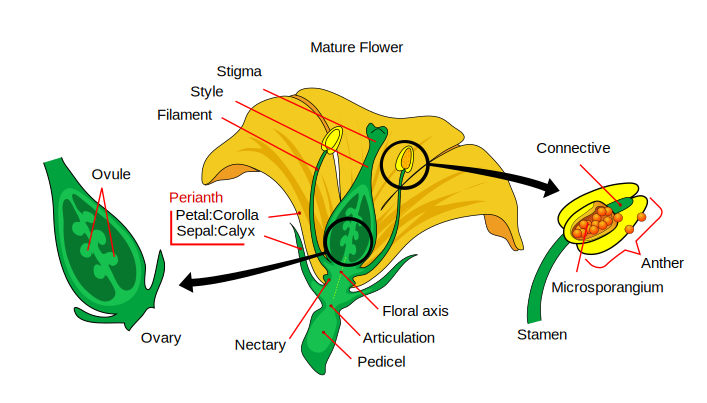
\includegraphics[width=0.7\linewidth]{./figures/plants/mature_flower} 

}

\caption{\href{https://commons.wikimedia.org/wiki/File:Mature_flower_diagram.svg}{Anatomy of the flower.}}\label{fig:flower}
\end{figure}

The characteristic feature of angiosperms is the flower. Flowers show remarkable variation in form and elaboration, and provide the most trustworthy external characteristics for establishing relationships among angiosperm species. The function of the flower is to ensure fertilization of the ovule and development of fruit containing seeds. The floral apparatus may arise terminally on a shoot or from the axil of a leaf (where the petiole attaches to the stem). Occasionally, as in violets, a flower arises singly in the axil of an ordinary foliage-leaf. More typically, the flower-bearing portion of the plant is sharply distinguished from the foliage-bearing or vegetative portion, and forms a more or less elaborate branch-system called an inflorescence.



\begin{figure}

{\centering 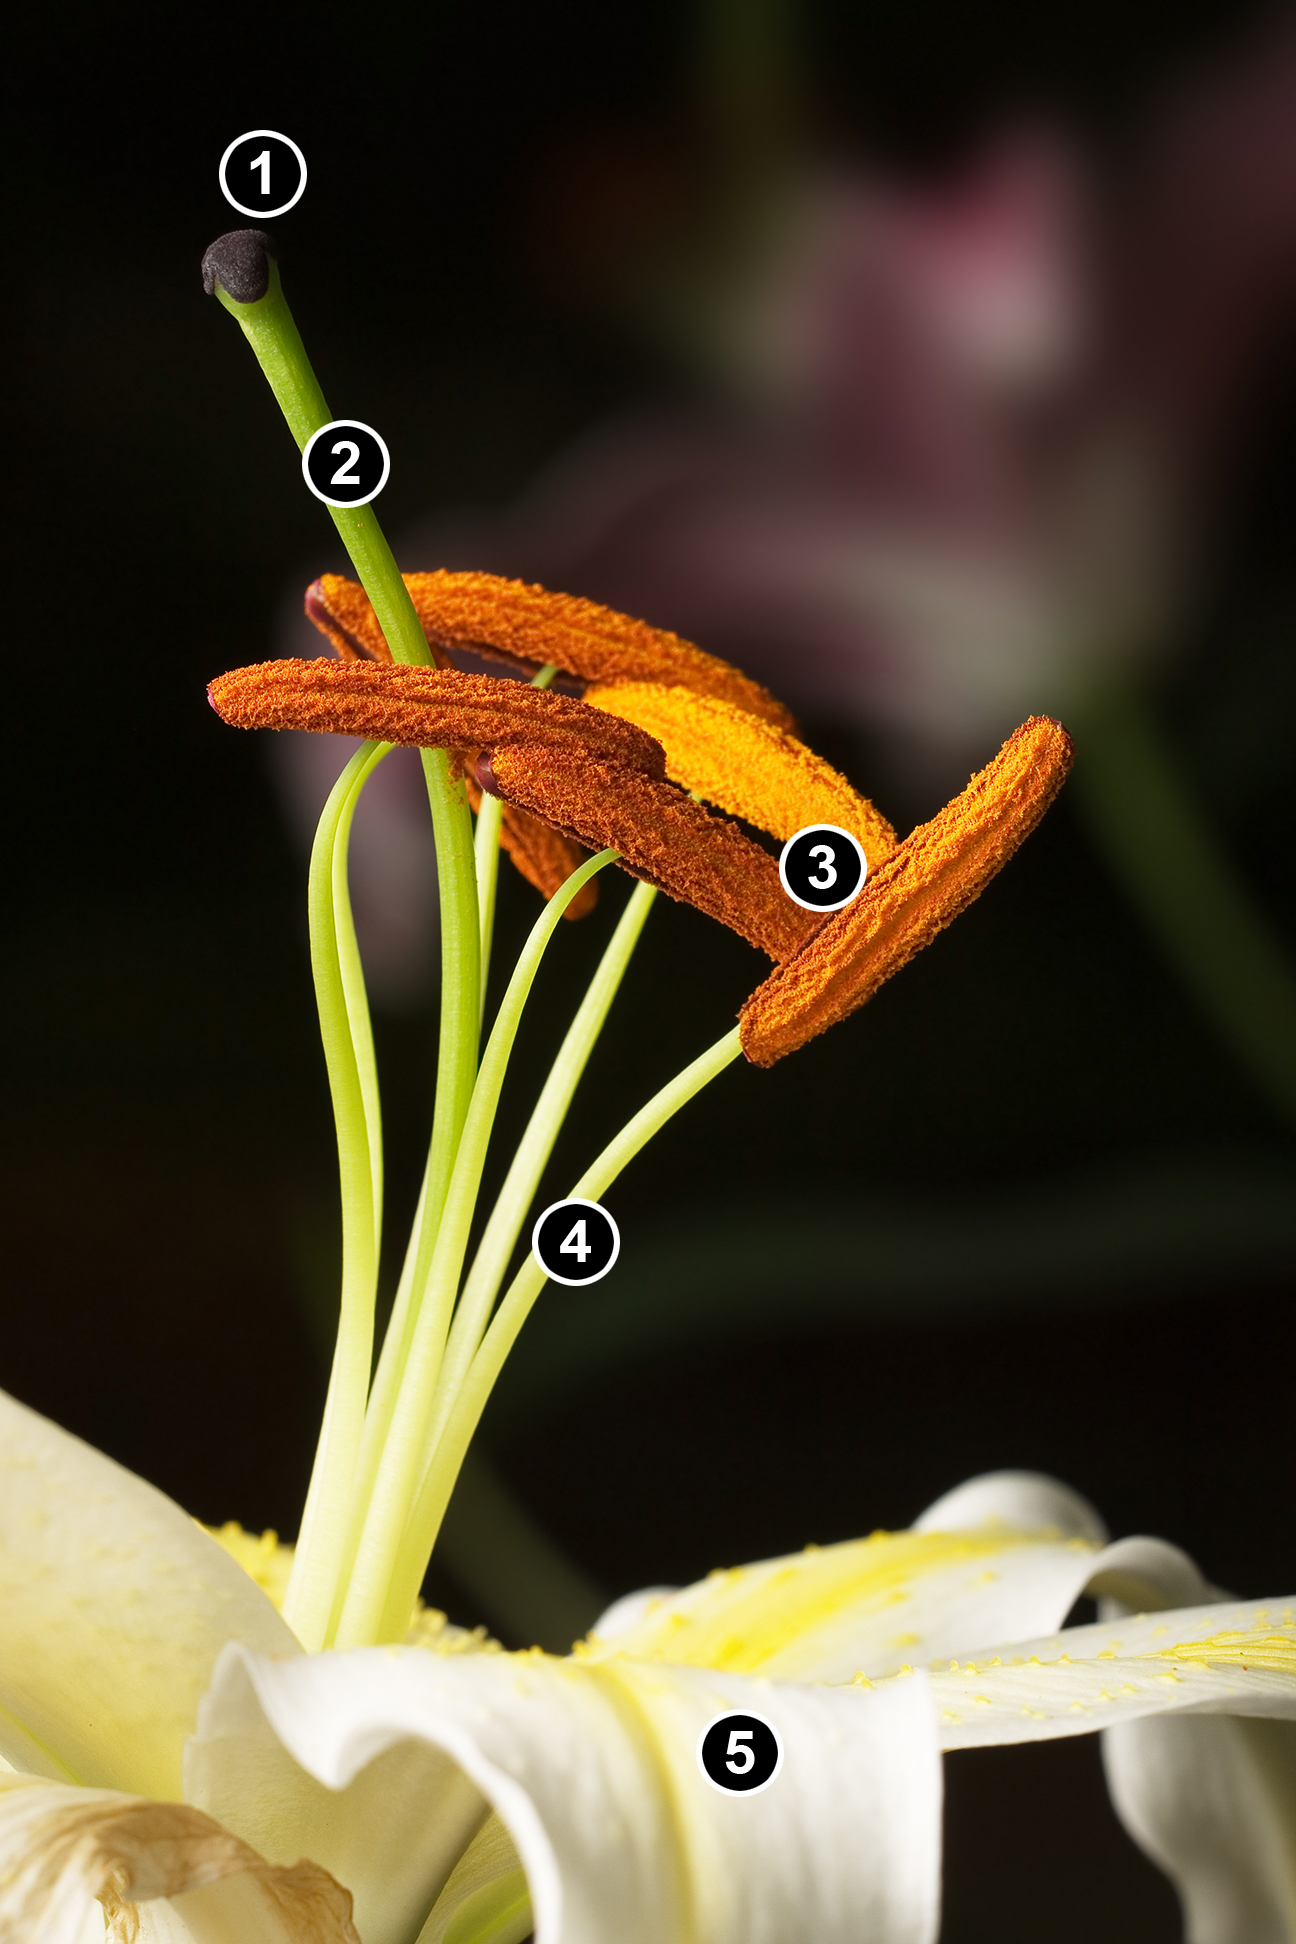
\includegraphics[width=0.7\linewidth]{./figures/plants/Lillium_Stamens} 

}

\caption{\href{https://commons.wikimedia.org/wiki/File:Lillium_Stamens.jpg}{Reproductive parts of Easter Lily (Lilium longiflorum).}1. Stigma, 2. Style, 3. Stamens, 4. Filament, 5. Petal}\label{fig:lilistamen}
\end{figure}

There are two kinds of reproductive cells produced by flowers. Microspores, which will divide to become pollen grains, are the ``male'' cells and are borne in the stamens (or microsporophylls). The ``female'' cells called megaspores, which will divide to become the egg cell (megagametogenesis), are contained in the ovule and enclosed in the carpel (or megasporophyll).

The flower may consist only of these parts, as in willow, where each flower comprises only a few stamens or two carpels. Usually, other structures are present and serve to protect the sporophylls and to form an envelope attractive to pollinators. The individual members of these surrounding structures are known as sepals and petals (or tepals in flowers such as Magnolia where sepals and petals are not distinguishable from each other). The outer series (calyx of sepals) is usually green and leaf-like, and functions to protect the rest of the flower, especially the bud. The inner series (corolla of petals) is, in general, white or brightly colored, and is more delicate in structure. It functions to attract insect or bird pollinators. Attraction is effected by color, scent, and nectar, which may be secreted in some part of the flower. The characteristics that attract pollinators account for the popularity of flowers and flowering plants among humans.

While the majority of flowers are perfect or hermaphrodite (having both pollen and ovule producing parts in the same flower structure), flowering plants have developed numerous morphological and physiological mechanisms to reduce or prevent self-fertilization. Heteromorphic flowers have short carpels and long stamens, or vice versa, so animal pollinators cannot easily transfer pollen to the pistil (receptive part of the carpel). Homomorphic flowers may employ a biochemical (physiological) mechanism called self-incompatibility to discriminate between self and non-self pollen grains. In other species, the male and female parts are morphologically separated, developing on different flowers.

The botanical term ``Angiosperm'', from the Ancient Greek ἀγγεῖον, angeíon (bottle, vessel) and σπέρμα, sperma (seed), was coined in the form Angiospermae by Paul Hermann in 1690, as the name of one of his primary divisions of the plant kingdom. This included flowering plants possessing seeds enclosed in capsules, distinguished from his Gymnospermae, or flowering plants with achenial or schizo-carpic fruits, the whole fruit or each of its pieces being here regarded as a seed and naked. The term and its antonym were maintained by Carl Linnaeus with the same sense, but with restricted application, in the names of the orders of his class Didynamia. Its use with any approach to its modern scope became possible only after 1827, when Robert Brown established the existence of truly naked ovules in the Cycadeae and Coniferae, and applied to them the name Gymnosperms. From that time onward, as long as these Gymnosperms were, as was usual, reckoned as dicotyledonous flowering plants, the term Angiosperm was used antithetically by botanical writers, with varying scope, as a group-name for other dicotyledonous plants.

In 1851, Hofmeister discovered the changes occurring in the embryo-sac of flowering plants, and determined the correct relationships of these to the Cryptogamia. This fixed the position of Gymnosperms as a class distinct from Dicotyledons, and the term Angiosperm then gradually came to be accepted as the suitable designation for the whole of the flowering plants other than Gymnosperms, including the classes of Dicotyledons and Monocotyledons. This is the sense in which the term is used today.

In most taxonomies, the flowering plants are treated as a coherent group. The most popular descriptive name has been Angiospermae (Angiosperms), with Anthophyta (``flowering plants'') a second choice. These names are not linked to any rank. The Wettstein system and the Engler system use the name Angiospermae, at the assigned rank of subdivision. The Reveal system treated flowering plants as subdivision Magnoliophytina, but later split it to Magnoliopsida, Liliopsida, and Rosopsida. The Takhtajan system and Cronquist system treat this group at the rank of division, leading to the name Magnoliophyta (from the family name Magnoliaceae). The Dahlgren system and Thorne system (1992) treat this group at the rank of class, leading to the name Magnoliopsida. The APG system of 1998, and the later 2003 and 2009 revisions, treat the flowering plants as a clade called angiosperms without a formal botanical name. A formal classification was published alongside the 2009 revision in which the flowering plants form the Subclass Magnoliidae.

The internal classification of this group has undergone considerable revision. The Cronquist system, proposed by Arthur Cronquist in 1968 and published in its full form in 1981, is still widely used but is no longer believed to accurately reflect phylogeny. A consensus about how the flowering plants should be arranged has recently begun to emerge through the work of the Angiosperm Phylogeny Group (APG), which published an influential reclassification of the angiosperms in 1998. Updates incorporating more recent research were published as the APG II system in 2003, the APG III system in 2009, and the APG IV system in 2016.

Traditionally, the flowering plants are divided into two groups,

\begin{itemize}
\tightlist
\item
  Dicotyledoneae or Magnoliopsida
\item
  Monocotyledoneae or Liliopsida
\end{itemize}

which in the Cronquist system are called Magnoliopsida (at the rank of class, formed from the family name Magnoliaceae) and Liliopsida (at the rank of class, formed from the family name Liliaceae). Other descriptive names allowed by Article 16 of the ICBN include Dicotyledones or Dicotyledoneae, and Monocotyledones or Monocotyledoneae, which have a long history of use. In English a member of either group may be called a dicotyledon (plural dicotyledons) and monocotyledon (plural monocotyledons), or abbreviated, as dicot (plural dicots) and monocot (plural monocots). These names derive from the observation that the dicots most often have two cotyledons, or embryonic leaves, within each seed. The monocots usually have only one, but the rule is not absolute either way. From a broad diagnostic point of view, the number of cotyledons is neither a particularly handy, nor a reliable character.

Recent studies, as by the APG, show that the monocots form a monophyletic group (clade) but that the dicots do not (they are paraphyletic). Nevertheless, the majority of dicot species do form a monophyletic group, called the eudicots or tricolpates. Of the remaining dicot species, most belong to a third major clade known as the magnoliids, containing about 9,000 species. The rest include a paraphyletic grouping of early branching taxa known collectively as the basal angiosperms, plus the families Ceratophyllaceae and Chloranthaceae.

Fossilized spores suggest that land plants (embryophytes) have existed for at least 475 million years. Early land plants reproduced sexually with flagellated, swimming sperm, like the green algae from which they evolved. An adaptation to terrestrialization was the development of upright meiosporangia for dispersal by spores to new habitats. This feature is lacking in the descendants of their nearest algal relatives, the Charophycean green algae. A later terrestrial adaptation took place with retention of the delicate, avascular sexual stage, the gametophyte, within the tissues of the vascular sporophyte. This occurred by spore germination within sporangia rather than spore release, as in non-seed plants. A current example of how this might have happened can be seen in the precocious spore germination in Selaginella, the spike-moss. The result for the ancestors of angiosperms was enclosing them in a case, the seed.

The apparently sudden appearance of nearly modern flowers in the fossil record initially posed such a problem for the theory of evolution that Charles Darwin called it an ``abominable mystery''. However, the fossil record has considerably grown since the time of Darwin, and recently discovered angiosperm fossils such as Archaefructus, along with further discoveries of fossil gymnosperms, suggest how angiosperm characteristics may have been acquired in a series of steps. Several groups of extinct gymnosperms, in particular seed ferns, have been proposed as the ancestors of flowering plants, but there is no continuous fossil evidence showing exactly how flowers evolved. Some older fossils, such as the upper Triassic Sanmiguelia, have been suggested.



\begin{figure}

{\centering 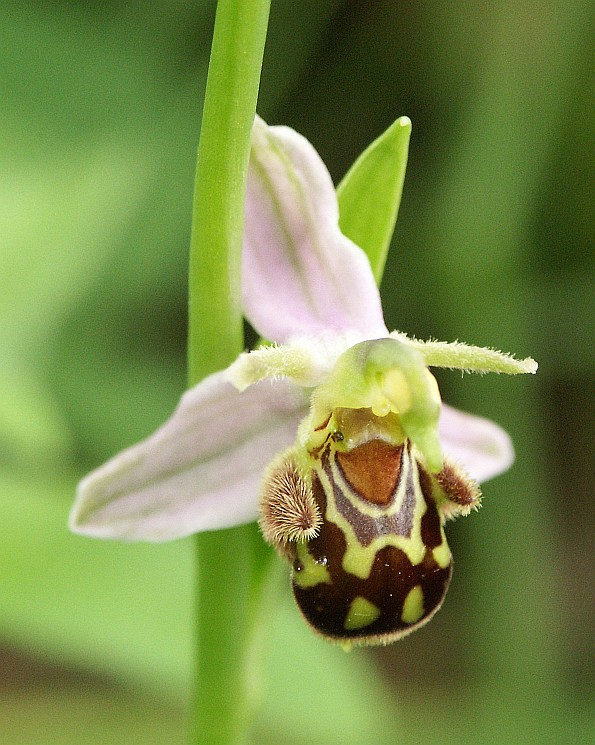
\includegraphics[width=0.7\linewidth]{./figures/plants/Ophrys_apifera_flower1} 

}

\caption{\href{https://commons.wikimedia.org/wiki/File:Ophrys_apifera_flower1.jpg}{A Bee orchid} has evolved over many generations to better mimic a female bee to attract male bees as pollinators.}\label{fig:beeorchid}
\end{figure}

The first seed bearing plants, like the ginkgo, and conifers (such as pines and firs), did not produce flowers. The pollen grains (male gametophytes) of Ginkgo and cycads produce a pair of flagellated, mobile sperm cells that ``swim'' down the developing pollen tube to the female and her eggs.

Oleanane, a secondary metabolite produced by many flowering plants, has been found in Permian deposits of that age together with fossils of gigantopterids. Gigantopterids are a group of extinct seed plants that share many morphological traits with flowering plants, although they are not known to have been flowering plants themselves.

Based on current evidence, some propose that the ancestors of the angiosperms diverged from an unknown group of gymnosperms in the Triassic period (245--202 million years ago). Fossil angiosperm-like pollen from the Middle Triassic (247.2--242.0 Ma) suggests an older date for their origin. A close relationship between angiosperms and gnetophytes, proposed on the basis of morphological evidence, has more recently been disputed on the basis of molecular evidence that suggest gnetophytes are instead more closely related to other gymnosperms.

The fossil plant species Nanjinganthus dendrostyla from Early Jurassic China seems to share many exclusively angiosperm features, such as a thickened receptacle with ovules, and thus might represent a crown-group or a stem-group angiosperm. However, the interpretation of the structures in this fossils are highly contested.

The evolution of seed plants and later angiosperms appears to be the result of two distinct rounds of whole genome duplication events. These occurred at 319 million years ago and 192 million years ago. Another possible whole genome duplication event at 160 million years ago perhaps created the ancestral line that led to all modern flowering plants. That event was studied by sequencing the genome of an ancient flowering plant, Amborella trichopoda, and directly addresses Darwin's ``abominable mystery''.

One study has suggested that the early-middle Jurassic plant Schmeissneria, traditionally considered a type of ginkgo, may be the earliest known angiosperm, or at least a close relative.

It has been proposed that the swift rise of angiosperms to dominance was facilitated by a reduction in their genome size. During the early Cretaceous period, only angiosperms underwent rapid genome downsizing, while genome sizes of ferns and gymnosperms remained unchanged. Smaller genomes---and smaller nuclei---allow for faster rates of cell division and smaller cells. Thus, species with smaller genomes can pack more, smaller cells---in particular veins and stomata---into a given leaf volume. Genome downsizing therefore facilitated higher rates of leaf gas exchange (transpiration and photosynthesis) and faster rates of growth. This would have countered some of the negative physiological effects of genome duplications, facilitated increased uptake of carbon dioxide despite concurrent declines in atmospheric CO\textsubscript{2}) concentrations, and allowed the flowering plants to outcompete other land plants.

The earliest known macrofossil confidently identified as an angiosperm, Archaefructus liaoningensis, is dated to about 125 million years BP (the Cretaceous period), whereas pollen considered to be of angiosperm origin takes the fossil record back to about 130 million years BP, with Montsechia representing the earliest flower at that time. In 2018, scientists reported that the earliest flowers began about 180 million years ago, 50 million years earlier than thought earlier. Nonetheless, circumstantial chemical evidence has been found for the existence of angiosperms as early as 250 million years ago .

In 2013 flowers encased in amber were found and dated 100 million years before present. The amber had frozen the act of sexual reproduction in the process of taking place. Microscopic images showed tubes growing out of pollen and penetrating the flower's stigma. The pollen was sticky, suggesting it was carried by insects. In August 2017, scientists presented a detailed description and 3D model image of what the first flower possibly looked like, and presented the hypothesis that it may have lived about 140 million years ago. A Bayesian analysis of 52 angiosperm taxa suggested that the crown group of angiosperms evolved between 178 million years ago and 198 million years ago.

Recent DNA analysis based on molecular systematics showed that Amborella trichopoda, found on the Pacific island of New Caledonia, belongs to a sister group of the other flowering plants, and morphological studies suggest that it has features that may have been characteristic of the earliest flowering plants. The orders Amborellales, Nymphaeales, and Austrobaileyales diverged as separate lineages from the remaining angiosperm clade at a very early stage in flowering plant evolution.

The great angiosperm radiation, when a great diversity of angiosperms appears in the fossil record, occurred in the mid-Cretaceous (approximately 100 million years ago). However, a study in 2007 estimated that the division of the five most recent (the genus Ceratophyllum, the family Chloranthaceae, the eudicots, the magnoliids, and the monocots) of the eight main groups occurred around 140 million years ago. It is generally assumed that the function of flowers, from the start, was to involve mobile animals in their reproduction processes. That is, pollen can be scattered even if the flower is not brightly colored or oddly shaped in a way that attracts animals; however, by expending the energy required to create such traits, angiosperms can enlist the aid of animals and, thus, reproduce more efficiently.

Island genetics provides one proposed explanation for the sudden, fully developed appearance of flowering plants. Island genetics is believed to be a common source of speciation in general, especially when it comes to radical adaptations that seem to have required inferior transitional forms. Flowering plants may have evolved in an isolated setting like an island or island chain, where the plants bearing them were able to develop a highly specialized relationship with some specific animal (a wasp, for example). Such a relationship, with a hypothetical wasp carrying pollen from one plant to another much the way fig wasps do today, could result in the development of a high degree of specialization in both the plant(s) and their partners. Note that the wasp example is not incidental; bees, which, it is postulated, evolved specifically due to mutualistic plant relationships, are descended from wasps.

Animals are also involved in the distribution of seeds. Fruit, which is formed by the enlargement of flower parts, is frequently a seed-dispersal tool that attracts animals to eat or otherwise disturb it, incidentally scattering the seeds it contains (see frugivory). Although many such mutualistic relationships remain too fragile to survive competition and to spread widely, flowering proved to be an unusually effective means of reproduction, spreading (whatever its origin) to become the dominant form of land plant life.

Flower ontogeny uses a combination of genes normally responsible for forming new shoots. The most primitive flowers probably had a variable number of flower parts, often separate from (but in contact with) each other. The flowers tended to grow in a spiral pattern, to be bisexual (in plants, this means both male and female parts on the same flower), and to be dominated by the ovary (female part). As flowers evolved, some variations developed parts fused together, with a much more specific number and design, and with either specific sexes per flower or plant or at least ``ovary-inferior''. Flower evolution continues to the present day; modern flowers have been so profoundly influenced by humans that some of them cannot be pollinated in nature. Many modern domesticated flower species were formerly simple weeds, which sprouted only when the ground was disturbed. Some of them tended to grow with human crops, perhaps already having symbiotic companion plant relationships with them, and the prettiest did not get plucked because of their beauty, developing a dependence upon and special adaptation to human affection.

A few paleontologists have also proposed that flowering plants, or angiosperms, might have evolved due to interactions with dinosaurs. One of the idea's strongest proponents is Robert T. Bakker. He proposes that herbivorous dinosaurs, with their eating habits, provided a selective pressure on plants, for which adaptations either succeeded in deterring or coping with predation by herbivores.

By the late Cretaceous, angiosperms appear to have dominated environments formerly occupied by ferns and cycadophytes, but large canopy-forming trees replaced conifers as the dominant trees only close to the end of the Cretaceous 66 million years ago or even later, at the beginning of the Tertiary. The radiation of herbaceous angiosperms occurred much later. Yet, many fossil plants recognizable as belonging to modern families (including beech, oak, maple, and magnolia) had already appeared by the late Cretaceous. Flowering plants appeared in Australia about 126 million years ago. This also pushed the age of ancient Australian vertebrates, in what was then a south polar continent, to 126-110 million years old.

\hypertarget{fertilization-and-embryogenesis}{%
\subsection{Fertilization and Embryogenesis}\label{fertilization-and-embryogenesis}}

Double fertilization refers to a process in which two sperm cells fertilize cells in the ovule. This process begins when a pollen grain adheres to the stigma of the pistil (female reproductive structure), germinates, and grows a long pollen tube. While this pollen tube is growing, a haploid generative cell travels down the tube behind the tube nucleus. The generative cell divides by mitosis to produce two haploid (n) sperm cells. As the pollen tube grows, it makes its way from the stigma, down the style and into the ovary. Here the pollen tube reaches the micropyle of the ovule and digests its way into one of the synergids, releasing its contents (which include the sperm cells). The synergid that the cells were released into degenerates and one sperm makes its way to fertilize the egg cell, producing a diploid (2n) zygote. The second sperm cell fuses with both central cell nuclei, producing a triploid (3n) cell. As the zygote develops into an embryo, the triploid cell develops into the endosperm, which serves as the embryo's food supply. The ovary will now develop into a fruit and the ovule will develop into a seed.

As the development of embryo and endosperm proceeds within the embryo sac, the sac wall enlarges and combines with the nucellus (which is likewise enlarging) and the integument to form the seed coat. The ovary wall develops to form the fruit or pericarp, whose form is closely associated with type of seed dispersal system.

Frequently, the influence of fertilization is felt beyond the ovary, and other parts of the flower take part in the formation of the fruit, e.g., the floral receptacle in the apple, strawberry, and others.

The character of the seed coat bears a definite relation to that of the fruit. They protect the embryo and aid in dissemination; they may also directly promote germination. Among plants with indehiscent fruits, in general, the fruit provides protection for the embryo and secures dissemination. In this case, the seed coat is only slightly developed. If the fruit is dehiscent and the seed is exposed, in general, the seed-coat is well developed, and must discharge the functions otherwise executed by the fruit.

Flowering plants generate gametes using a specialized cell division called meiosis. Meiosis takes place in the ovule (a structure within the ovary that is located within the pistil at the center of the flower) (see diagram labeled ``Angiosperm lifecycle''). A diploid cell (megaspore mother cell) in the ovule undergoes meiosis (involving two successive cell divisions) to produce four cells (megaspores) with haploid nuclei. It is thought that the basal chromosome number in angiosperms is n = 7. One of these four cells (megaspore) then undergoes three successive mitotic divisions to produce an immature embryo sac (megagametophyte) with eight haploid nuclei. Next, these nuclei are segregated into separate cells by cytokinesis to producing 3 antipodal cells, 2 synergid cells and an egg cell. Two polar nuclei are left in the central cell of the embryo sac.

Pollen is also produced by meiosis in the male anther (microsporangium). During meiosis, a diploid microspore mother cell undergoes two successive meiotic divisions to produce 4 haploid cells (microspores or male gametes). Each of these microspores, after further mitoses, becomes a pollen grain (microgametophyte) containing two haploid generative (sperm) cells and a tube nucleus. When a pollen grain makes contact with the female stigma, the pollen grain forms a pollen tube that grows down the style into the ovary. In the act of fertilization, a male sperm nucleus fuses with the female egg nucleus to form a diploid zygote that can then develop into an embryo within the newly forming seed. Upon germination of the seed, a new plant can grow and mature.



\begin{figure}

{\centering 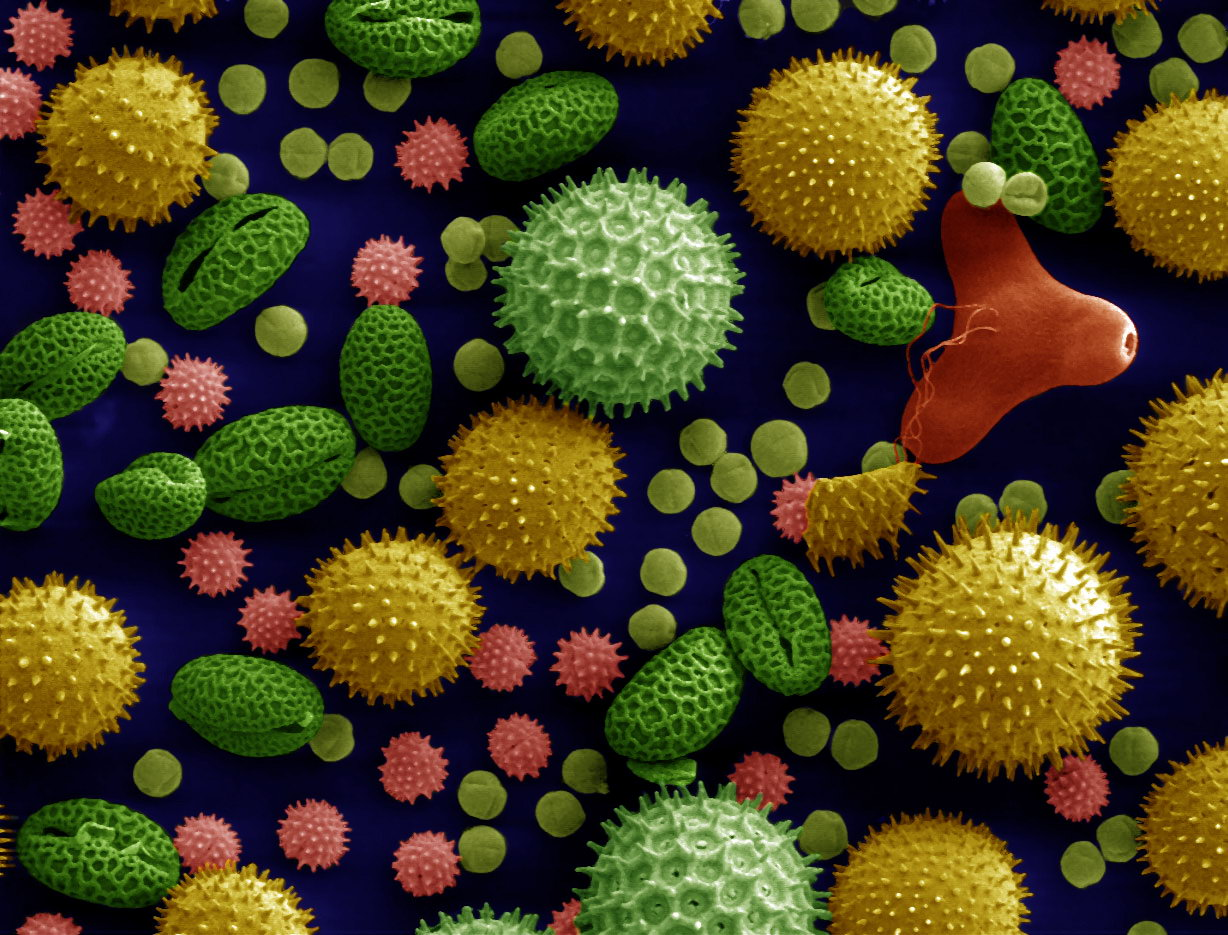
\includegraphics[width=0.7\linewidth]{./figures/plants/Misc_pollen_colorized} 

}

\caption{\href{https://commons.wikimedia.org/wiki/File:Misc_pollen_colorized.jpg}{Scanning electron microscope image (500x magnification) of pollen grains from a variety of common plants:} sunflower (\emph{Helianthus annuus}), morning glory (\emph{Ipomoea purpurea}), prairie hollyhock (\emph{Sidalcea malviflora}), oriental lily (\emph{Lilium auratum}), evening primrose (\emph{Oenothera fruticosa}), and castor bean (\emph{Ricinus communis}).The image is magnified some x500, so the bean shaped grain in the bottom left corner is about 50 μm long. The colors are computer-generated.}\label{fig:miscpollen}
\end{figure}

The adaptive function of meiosis is currently a matter of debate. A key event during meiosis in a diploid cell is the pairing of homologous chromosomes and homologous recombination (the exchange of genetic information) between homologous chromosomes. This process promotes the production of increased genetic diversity among progeny and the recombinational repair of damages in the DNA to be passed on to progeny. To explain the adaptive function of meiosis in flowering plants, some authors emphasize diversity and others emphasize DNA repair.

\hypertarget{plant-anatomy}{%
\section{Plant Anatomy}\label{plant-anatomy}}

Plant anatomy or phytotomy is the general term for the study of the internal structure of plants. Originally it included plant morphology, the description of the physical form and external structure of plants, but since the mid-20th century plant anatomy has been considered a separate field referring only to internal plant structure. Plant anatomy is now frequently investigated at the cellular level, and often involves the sectioning of tissues and microscopy.

Some studies of plant anatomy use a systems approach, organized on the basis of the plant's activities, such as nutrient transport, flowering, pollination, embryogenesis or seed development. Others are more classically divided into the following structural categories:

\begin{itemize}
\tightlist
\item
  Flower anatomy, including study of the Calyx, Corolla, Androecium, and Gynoecium
\item
  Leaf anatomy, including study of the Epidermis, stomata and Palisade cells
\item
  Stem anatomy, including Stem structure and vascular tissues, buds and shoot apex
\item
  Fruit/Seed anatomy, including structure of the Ovule, Seed, Pericarp and Accessory fruit
\item
  Wood anatomy, including structure of the Bark, Cork, Xylem, Phloem, Vascular cambium, Heartwood and sapwood and branch collar
\item
  Root anatomy, including structure of the Root, root tip, endodermis
\end{itemize}

Organs of plants can be divided into vegetative and reproductive. Vegetative plant organs include roots, stems, and leaves. The reproductive organs are variable. In flowering plants, they are represented by the flower, seed and fruit. In conifers, the organ that bears the reproductive structures is called a cone. In other divisions (phyla) of plants, the reproductive organs are called strobili, in Lycopodiophyta, or simply gametophores in mosses.

The vegetative organs are essential for maintaining the life of a plant. While there can be 11 organ systems in animals, there are far fewer in plants, where some perform the vital functions, such as photosynthesis, while the reproductive organs are essential in reproduction. However, if there is asexual vegetative reproduction, the vegetative organs are those that create the new generation of plants (see clonal colony).

\hypertarget{plant-tissues}{%
\section{Plant Tissues}\label{plant-tissues}}

In plant anatomy, tissues are categorized broadly into three tissue systems: the epidermis, the ground tissue, and the vascular tissue.

\begin{itemize}
\tightlist
\item
  Epidermis - Cells forming the outer surface of the leaves and of the young plant body.
\item
  Vascular tissue - The primary components of vascular tissue are the xylem and phloem. These transport fluids and nutrients internally.
\item
  Ground tissue - Ground tissue is less differentiated than other tissues. Ground tissue manufactures nutrients by photosynthesis and stores reserve nutrients.
\end{itemize}

Plant tissues can also be divided differently into two types:

\begin{enumerate}
\def\labelenumi{\arabic{enumi}.}
\tightlist
\item
  Meristematic tissues
\item
  Permanent tissues.
\end{enumerate}

\hypertarget{meristematic-tissues}{%
\subsection{Meristematic Tissues}\label{meristematic-tissues}}

Meristematic tissue consists of actively dividing cells, and leads to increase in length and thickness of the plant. The primary growth of a plant occurs only in certain, specific regions, such as in the tips of stems or roots. It is in these regions that meristematic tissues are present. Cells in these tissues are roughly spherical or polyhedral, to rectangular in shape, and have thin cell walls. New cells produced by meristem are initially those of meristem itself, but as the new cells grow and mature, their characteristics slowly change and they become differentiated as components of the region of occurrence of meristematic tissues, being classified as:

\begin{itemize}
\tightlist
\item
  Apical meristem - It is present at the growing tips of stems and roots and increases the length of the stem and root. They form growing parts at the apices of roots and stems and are responsible for the increase in length, also called primary growth. This meristem is responsible for the linear growth of an organ.
\item
  Lateral meristem - This meristem consists of cells which mainly divide in one plane and cause the organ to increase in diameter and growth. Lateral meristem usually occurs beneath the bark of the tree in the form of Cork Cambium and in vascular bundles of dicots in the form of vascular cambium. The activity of this cambium results in the formation of secondary growth.
\item
  Intercalary meristem - This meristem is located in between permanent tissues. It is usually present at the base of the node, internode and on leaf base. They are responsible for growth in length of the plant and increasing the size of the internode. They result in branch formation and growth.
\end{itemize}

The cells of meristematic tissues are similar in structure and have thin and elastic primary cell wall made up of cellulose. They are compactly arranged without inter-cellular spaces between them. Each cell contains a dense cytoplasm and a prominent nucleus. The dense protoplasm of meristematic cells contains very few vacuoles. Normally the meristematic cells are oval, polygonal or rectangular in shape.

Meristematic tissue cells have a large nucleus with small or no vacuoles as they have no need to store anything, opposed to their function of multiplying and increasing the girth and length of the plant, and no intercellular spaces.

\hypertarget{permanent-tissues}{%
\subsection{Permanent Tissues}\label{permanent-tissues}}

Permanent tissues may be defined as a group of living or dead cells formed by meristematic tissue and have lost their ability to divide and have permanently placed at fixed positions in the plant body. Meristematic tissues that take up a specific role lose the ability to divide. This process of taking up a permanent shape, size and a function is called cellular differentiation. Cells of meristematic tissue differentiate to form different types of permanent tissues. There are 3 types of permanent tissues:

\begin{enumerate}
\def\labelenumi{\arabic{enumi}.}
\tightlist
\item
  simple permanent tissues
\item
  complex permanent tissues
\item
  special or secretory tissues (glandular).
\end{enumerate}

Simple Permanent tissues

A group of cells which are similar in origin; similar in structure and similar in function are called simple permanent tissue. They are of three types:

\begin{enumerate}
\def\labelenumi{\arabic{enumi}.}
\tightlist
\item
  Parenchyma
\item
  Collenchyma
\item
  Sclerenchyma
\end{enumerate}

\hypertarget{parenchyma}{%
\subsection{Parenchyma}\label{parenchyma}}

Parenchyma (para - `beside'; infusion - `tissue') is the bulk of a substance. In plants, it consists of relatively unspecialized living cells with thin cell walls that are usually loosely packed so that intercellular spaces are found between cells of this tissue. These are generally isodiametric, in shape. They contain small number of vacuoles or sometimes they even may not contain any vacuole. Even if they do so the vacuole is of much smaller size than of normal animal cells. This tissue provides support to plants and also stores food. Chlorenchyma is a special type of parenchyma that contains chlorophyll and performs photosynthesis. In aquatic plants, aerenchyma tissues, or large air cavities, give support to float on water by making them buoyant. Parenchyma cells called idioblasts have metabolic waste. Spindle shape fiber also contained into this cell to support them and known as prosenchyma, succulent parenchyma also noted. In xerophytes, parenchyma tissues store water.

\hypertarget{collenchyma}{%
\subsection{Collenchyma}\label{collenchyma}}

Collenchyma is Greek word where ``Colla'' means gum and ``enchyma'' means infusion. It is a living tissue of primary body like Parenchyma. Cells are thin-walled but possess thickening of cellulose, water and pectin substances (pectocellulose) at the corners where a number of cells join together. This tissue gives tensile strength to the plant and the cells are compactly arranged and have very little inter-cellular spaces. It occurs chiefly in hypodermis of stems and leaves. It is absent in monocots and in roots. Sometimes it contains chlorophyll which can help them photosynthesize.

Collenchymatous tissue acts as a supporting tissue in stems of young plants. It provides mechanical support, elasticity, and tensile strength to the plant body. It helps in manufacturing sugar and storing it as starch. It is present in the margin of leaves and resists tearing effect of the wind.

\hypertarget{sclerenchyma}{%
\subsection{Sclerenchyma}\label{sclerenchyma}}

Sclerenchyma is Greek word where ``Sclero-'' means hard and ``enchyma'' means infusion. This tissue consists of thick-walled, dead cells and protoplasm is negligible. These cells have hard and extremely thick secondary walls due to uniform distribution and high secretion of lignin and have a function of providing mechanical support. They do not have inter-molecular space between them. Lignin deposition is so thick that the cell walls become strong, rigid and impermeable to water which is also known as a stone cell or sclereids. These tissues are mainly of two types: sclerenchyma fiber and sclereids. Sclerenchyma fiber cells have a narrow lumen and are long, narrow and unicellular. Fibers are elongated cells that are strong and flexible, often used in ropes. Sclereids have extremely thick cell walls and are brittle, and are found in nutshells and legumes.

\hypertarget{epidermis}{%
\subsection{Epidermis}\label{epidermis}}

The entire surface of the plant consists of a single layer of cells called epidermis or surface tissue. The entire surface of the plant has this outer layer of the epidermis. Hence it is also called surface tissue. Most of the epidermal cells are relatively flat. The outer and lateral walls of the cell are often thicker than the inner walls. The cells form a continuous sheet without intercellular spaces. It protects all parts of the plant. The outer epidermis is coated with a waxy thick layer called cuticle which prevents loss of water. The epidermis also consists of stomata(singular:stoma) which helps in transpiration.

\hypertarget{complex-permanent-tissue}{%
\subsection{Complex Permanent Tissue}\label{complex-permanent-tissue}}

The complex tissue consists of more than one type of cells which work together as a unit. Complex tissues help in the transportation of organic material, water, and minerals up and down the plants. That is why it is also known as conducting and vascular tissue. The common types of complex permanent tissue are:

\begin{itemize}
\tightlist
\item
  Xylem or wood
\item
  Phloem or bast.
\end{itemize}

Xylem and phloem together form vascular bundles.

\hypertarget{xylem}{%
\subsection{Xylem}\label{xylem}}

Xylem consists of:

\begin{itemize}
\tightlist
\item
  Xylem tracheids
\item
  Xylem vessel
\item
  Xylem fibres or Xylem sclerenchyma
\item
  Xylem parenchyma
\end{itemize}

Xylem serves as a chief conducting tissue of vascular plants.

It is responsible for the conduction of water and mineral ions/salt. Xylem tissue is organised in a tube-like fashion along the main axes of stems and roots. It consists of a combination of parenchyma cells, fibers, vessels, tracheids, and ray cells. Longer tubes made up of individual cells are vessels tracheids, while vessel members are open at each end. Internally, there may be bars of wall material extending across the open space. These cells are joined end to end to form long tubes. Vessel members and tracheids are dead at maturity. Tracheids have thick secondary cell walls and are tapered at the ends. They do not have end openings such as the vessels. The tracheids end overlap with each other, with pairs of pits present. The pit pairs allow water to pass from cell to cell.

Though most conduction in xylem tissue is vertical, lateral conduction along the diameter of a stem is facilitated via rays. Rays are horizontal rows of long-living parenchyma cells that arise out of the vascular cambium. In trees and other woody plants, rays radiate out from the center of stems and roots and appear like spokes on a wheel in cross section. Rays, unlike vessel members and tracheids, are alive at functional maturity.

\hypertarget{phloem}{%
\subsection{Phloem}\label{phloem}}

Phloem consists of:

\begin{itemize}
\tightlist
\item
  Sieve tube
\item
  Companion cell
\item
  Phloem fibre
\item
  Phloem parenchyma.
\end{itemize}

Phloem is an equally important plant tissue as it also is part of the `plumbing system' of a plant. Primarily, phloem carries dissolved food substances throughout the plant. This conduction system is composed of sieve-tube member and companion cells, that are without secondary walls. The parent cells of the vascular cambium produce both xylem and phloem. This usually also includes fibers, parenchyma and ray cells. Sieve tubes are formed from sieve-tube members laid end to end. The end walls, unlike vessel members in xylem, do not have openings. The end walls, however, are full of small pores where cytoplasm extends from cell to cell. These porous connections are called sieve plates. In spite of the fact that their cytoplasm is actively involved in the conduction of food materials, sieve-tube members do not have nuclei at maturity. It is the companion cells that are nestled between sieve-tube members that function in some manner bringing about the conduction of food. Sieve-tube members that are alive contain a polymer called callose, a carbohydrate polymer, forming the callus pad/callus, the colourless substance that covers the sieve plate. Callose stays in solution as long as the cell contents are under pressure. Phloem transports food and materials in plants upwards and downwards as required.

\hypertarget{plant-cells}{%
\subsection{Plant cells}\label{plant-cells}}

Plant cells are typically distinguished by their large water-filled central vacuole, chloroplasts, and rigid cell walls that are made up of cellulose, hemicellulose, and pectin. Cell division is also characterized by the development of a phragmoplast for the construction of a cell plate in the late stages of cytokinesis. Just as in animals, plant cells differentiate and develop into multiple cell types. Totipotent meristematic cells can differentiate into vascular, storage, protective (e.g.~epidermal layer), or reproductive tissues, with more primitive plants lacking some tissue types.

\hypertarget{biochemistry-of-plants}{%
\section{Biochemistry of Plants}\label{biochemistry-of-plants}}

The chemical elements of which plants are constructed---principally carbon, oxygen, hydrogen, nitrogen, phosphorus, sulfur, etc.---are the same as for all other life forms animals, fungi, bacteria and even viruses. Only the details of the molecules into which they are assembled differs.

Despite this underlying similarity, plants produce a vast array of chemical compounds with unique properties which they use to cope with their environment. Pigments are used by plants to absorb or detect light, and are extracted by humans for use in dyes. Other plant products may be used for the manufacture of commercially important rubber or biofuel. Perhaps the most celebrated compounds from plants are those with pharmacological activity, such as salicylic acid from which aspirin is made, morphine, and digoxin. Drug companies spend billions of dollars each year researching plant compounds for potential medicinal benefits.

Plants require some nutrients, such as carbon and nitrogen, in large quantities to survive. Some nutrients are termed macronutrients, where the prefix macro- (large) refers to the quantity needed, not the size of the nutrient particles themselves. Other nutrients, called micronutrients, are required only in trace amounts for plants to remain healthy. Such micronutrients are usually absorbed as ions dissolved in water taken from the soil, though carnivorous plants acquire some of their micronutrients from captured prey.

The following tables list element nutrients essential to plants. Uses within plants are generalized.

\hypertarget{pigments}{%
\subsection{Pigments}\label{pigments}}

Among the most important molecules for plant function are the pigments. Plant pigments include a variety of different kinds of molecules, including porphyrins, carotenoids, and anthocyanins. All biological pigments selectively absorb certain wavelengths of light while reflecting others. The light that is absorbed may be used by the plant to power chemical reactions, while the reflected wavelengths of light determine the color the pigment appears to the eye.

Chlorophyll is the primary pigment in plants; it is a porphyrin that absorbs red and blue wavelengths of light while reflecting green. It is the presence and relative abundance of chlorophyll that gives plants their green color. All land plants and green algae possess two forms of this pigment: chlorophyll a and chlorophyll b. Kelps, diatoms, and other photosynthetic heterokonts contain chlorophyll c instead of b, red algae possess chlorophyll a. All chlorophylls serve as the primary means plants use to intercept light to fuel photosynthesis.

Carotenoids are red, orange, or yellow tetraterpenoids. They function as accessory pigments in plants, helping to fuel photosynthesis by gathering wavelengths of light not readily absorbed by chlorophyll. The most familiar carotenoids are carotene (an orange pigment found in carrots), lutein (a yellow pigment found in fruits and vegetables), and lycopene (the red pigment responsible for the color of tomatoes). Carotenoids have been shown to act as antioxidants and to promote healthy eyesight in humans.

Anthocyanins (literally ``flower blue'') are water-soluble flavonoid pigments that appear red to blue, according to pH. They occur in all tissues of higher plants, providing color in leaves, stems, roots, flowers, and fruits, though not always in sufficient quantities to be noticeable. Anthocyanins are most visible in the petals of flowers, where they may make up as much as 30\% of the dry weight of the tissue. They are also responsible for the purple color seen on the underside of tropical shade plants such as Tradescantia zebrina. In these plants, the anthocyanin catches light that has passed through the leaf and reflects it back towards regions bearing chlorophyll, in order to maximize the use of available light

Betalains are red or yellow pigments. Like anthocyanins they are water-soluble, but unlike anthocyanins they are indole-derived compounds synthesized from tyrosine. This class of pigments is found only in the Caryophyllales (including cactus and amaranth), and never co-occur in plants with anthocyanins. Betalains are responsible for the deep red color of beets, and are used commercially as food-coloring agents. Plant physiologists are uncertain of the function that betalains have in plants which possess them, but there is some preliminary evidence that they may have fungicidal properties.

\hypertarget{plant-hormones}{%
\subsection{Plant Hormones}\label{plant-hormones}}

Plants produce hormones and other growth regulators which act to signal a physiological response in their tissues. They also produce compounds such as phytochrome that are sensitive to light and which serve to trigger growth or development in response to environmental signals.

Plant hormones, known as plant growth regulators (PGRs) or phytohormones, are chemicals that regulate a plant's growth. According to a standard animal definition, hormones are signal molecules produced at specific locations, that occur in very low concentrations, and cause altered processes in target cells at other locations. Unlike animals, plants lack specific hormone-producing tissues or organs. Plant hormones are often not transported to other parts of the plant and production is not limited to specific locations.

Plant hormones are chemicals that in small amounts promote and influence the growth, development and differentiation of cells and tissues. Hormones are vital to plant growth; affecting processes in plants from flowering to seed development, dormancy, and germination. They regulate which tissues grow upwards and which grow downwards, leaf formation and stem growth, fruit development and ripening, as well as leaf abscission and even plant death.

The most important plant hormones are abscissic acid (ABA), auxins, ethylene, gibberellins, and cytokinins, though there are many other substances that serve to regulate plant physiology.

\hypertarget{photomorphogenesis}{%
\subsection{Photomorphogenesis}\label{photomorphogenesis}}

While most people know that light is important for photosynthesis in plants, few realize that plant sensitivity to light plays a role in the control of plant structural development (morphogenesis). The use of light to control structural development is called photomorphogenesis, and is dependent upon the presence of specialized photoreceptors, which are chemical pigments capable of absorbing specific wavelengths of light.

Plants use four kinds of photoreceptors: phytochrome, cryptochrome, a UV-B photoreceptor, and protochlorophyllide a. The first two of these, phytochrome and cryptochrome, are photoreceptor proteins, complex molecular structures formed by joining a protein with a light-sensitive pigment. Cryptochrome is also known as the UV-A photoreceptor, because it absorbs ultraviolet light in the long wave ``A'' region. The UV-B receptor is one or more compounds not yet identified with certainty, though some evidence suggests carotene or riboflavin as candidates. Protochlorophyllide a, as its name suggests, is a chemical precursor of chlorophyll.

The most studied of the photoreceptors in plants is phytochrome. It is sensitive to light in the red and far-red region of the visible spectrum. Many flowering plants use it to regulate the time of flowering based on the length of day and night (photoperiodism) and to set circadian rhythms. It also regulates other responses including the germination of seeds, elongation of seedlings, the size, shape and number of leaves, the synthesis of chlorophyll, and the straightening of the epicotyl or hypocotyl hook of dicot seedlings.

\hypertarget{photoperiodism}{%
\subsection{Photoperiodism}\label{photoperiodism}}

Many flowering plants use the pigment phytochrome to sense seasonal changes in day length, which they take as signals to flower. This sensitivity to day length is termed photoperiodism. Broadly speaking, flowering plants can be classified as long day plants, short day plants, or day neutral plants, depending on their particular response to changes in day length. Long day plants require a certain minimum length of daylight to starts flowering, so these plants flower in the spring or summer. Conversely, short day plants flower when the length of daylight falls below a certain critical level. Day neutral plants do not initiate flowering based on photoperiodism, though some may use temperature sensitivity (vernalization) instead.

Although a short day plant cannot flower during the long days of summer, it is not actually the period of light exposure that limits flowering. Rather, a short day plant requires a minimal length of uninterrupted darkness in each 24-hour period (a short daylength) before floral development can begin. It has been determined experimentally that a short day plant (long night) does not flower if a flash of phytochrome activating light is used on the plant during the night.

Plants make use of the phytochrome system to sense day length or photoperiod. This fact is utilized by florists and greenhouse gardeners to control and even induce flowering out of season, such as the Poinsettia.

\hypertarget{plant-secondary-metabolism}{%
\section{Plant Secondary Metabolism}\label{plant-secondary-metabolism}}

Secondary metabolism produces a large number of specialized compounds (estimated 200,000) that do not aid in the growth and development of plants but are required for the plant to survive in its environment. Secondary metabolism is connected to primary metabolism by using building blocks and biosynthetic enzymes derived from primary metabolism. Primary metabolism governs all basic physiological processes that allow a plant to grow and set seeds, by translating the genetic code into proteins, carbohydrates, and amino acids. Specialized compounds from secondary metabolism are essential for communicating with other organisms in mutualistic (e.g.~attraction of beneficial organisms such as pollinators) or antagonistic interactions (e.g.~deterrent against herbivores and pathogens). They further assist in coping with abiotic stress such as increased UV-radiation. The broad functional spectrum of specialized metabolism is still not fully understood. In any case, a good balance between products of primary and secondary metabolism is best for a plant's optimal growth and development as well as for its effective coping with often changing environmental conditions. Well known specialized compounds include alkaloids, polyphenols including flavonoids, and terpenoids. Humans use quite a lot of these compounds, or the plants from which they originate, for culinary, medicinal and nutraceutical purposes.

\hypertarget{tropisms-and-nastic-movements}{%
\section{Tropisms And Nastic Movements}\label{tropisms-and-nastic-movements}}

Plants may respond both to directional and non-directional stimuli. A response to a directional stimulus, such as gravity or sunlight, is called a tropism. A response to a nondirectional stimulus, such as temperature or humidity, is a nastic movement.

Tropisms in plants are the result of differential cell growth, in which the cells on one side of the plant elongates more than those on the other side, causing the part to bend toward the side with less growth. Among the common tropisms seen in plants is phototropism, the bending of the plant toward a source of light. Phototropism allows the plant to maximize light exposure in plants which require additional light for photosynthesis, or to minimize it in plants subjected to intense light and heat. Geotropism allows the roots of a plant to determine the direction of gravity and grow downwards. Tropisms generally result from an interaction between the environment and production of one or more plant hormones.

Nastic movements results from differential cell growth (e.g.~epinasty and hiponasty), or from changes in turgor pressure within plant tissues (e.g., nyctinasty), which may occur rapidly. A familiar example is thigmonasty (response to touch) in the Venus fly trap, a carnivorous plant. The traps consist of modified leaf blades which bear sensitive trigger hairs. When the hairs are touched by an insect or other animal, the leaf folds shut. This mechanism allows the plant to trap and digest small insects for additional nutrients. Although the trap is rapidly shut by changes in internal cell pressures, the leaf must grow slowly to reset for a second opportunity to trap insects.

\hypertarget{plant-reproduction}{%
\section{Plant Reproduction}\label{plant-reproduction}}

Plant reproduction is the production of new offspring in plants, which can be accomplished by sexual or asexual reproduction. Sexual reproduction produces offspring by the fusion of gametes, resulting in offspring genetically different from the parent or parents. Asexual reproduction produces new individuals without the fusion of gametes, genetically identical to the parent plants and each other, except when mutations occur.

\hypertarget{the-life-cycle-of-plants}{%
\subsection{The Life Cycle of Plants}\label{the-life-cycle-of-plants}}

Like all land plants (embryophytes), bryophytes have life cycles with alternation of generations. In each cycle, a haploid gametophyte, each of whose cells contains a fixed number of unpaired chromosomes, alternates with a diploid sporophyte, whose cell contain two sets of paired chromosomes. Gametophytes produce haploid sperm and eggs which fuse to form diploid zygotes that grow into sporophytes. Sporophytes produce haploid spores by meiosis, that grow into gametophytes.

Bryophytes are gametophyte dominant, meaning that the more prominent, longer-lived plant is the haploid gametophyte. The diploid sporophytes appear only occasionally and remain attached to and nutritionally dependent on the gametophyte. In bryophytes, the sporophytes are always unbranched and produce a single sporangium (spore producing capsule), but each gametophyte can give rise to several sporophytes at once.

The sporophyte develops differently in the three groups. Both mosses and hornworts have a meristem zone where cell division occur. In hornworts, the meristem starts at the base where the foot ends, and the division of cells is pushing the sporophyte body upwards. In mosses, the meristem is located between the capsule and the top of the stalk (seta), and produce cells downward, elongating the stalk and elevates the capsule. In liverworts the meristem is absent and the elongation of the sporophyte is caused almost exclusively by cell expansion.

Liverworts, mosses and hornworts spend most of their lives as gametophytes. Gametangia (gamete-producing organs), archegonia and antheridia, are produced on the gametophytes, sometimes at the tips of shoots, in the axils of leaves or hidden under thalli. Some bryophytes, such as the liverwort Marchantia, create elaborate structures to bear the gametangia that are called gametangiophores. Sperm are flagellated and must swim from the antheridia that produce them to archegonia which may be on a different plant. Arthropods can assist in transfer of sperm.

Fertilized eggs become zygotes, which develop into sporophyte embryos inside the archegonia. Mature sporophytes remain attached to the gametophyte. They consist of a stalk called a seta and a single sporangium or capsule. Inside the sporangium, haploid spores are produced by meiosis. These are dispersed, most commonly by wind, and if they land in a suitable environment can develop into a new gametophyte. Thus bryophytes disperse by a combination of swimming sperm and spores, in a manner similar to lycophytes, ferns and other cryptogams.

The arrangement of antheridia and archegonia on an individual bryophyte plant is usually constant within a species, although in some species it may depend on environmental conditions. The main division is between species in which the antheridia and archegonia occur on the same plant and those in which they occur on different plants. The term monoicous may be used where antheridia and archegonia occur on the same gametophyte and the term dioicous where they occur on different gametophytes.

In seed plants, ``monoecious'' is used where flowers with anthers (microsporangia) and flowers with ovules (megasporangia) occur on the same sporophyte and ``dioecious'' where they occur on different sporophytes. These terms occasionally may be used instead of ``monoicous'' and ``dioicous'' to describe bryophyte gametophytes. ``Monoecious'' and ``monoicous'' are both derived from the Greek for ``one house'', ``dioecious'' and ``dioicous'' from the Greek for two houses. The use of the ``oicy'' terminology refers to the gametophyte sexuality of bryophytes as distinct from the sporophyte sexuality of seed plants.

Monoicous plants are necessarily hermaphroditic, meaning that the same plant has both sexes. The exact arrangement of the antheridia and archegonia in monoicous plants varies. They may be borne on different shoots (autoicous or autoecious), on the same shoot but not together in a common structure (paroicous or paroecious), or together in a common ``inflorescence'' (synoicous or synoecious). Dioicous plants are unisexual, meaning that the same plant has only one sex. All four patterns (autoicous, paroicous, synoicous and dioicous) occur in species of the moss genus Bryum.

\hypertarget{asexual-reproduction-1}{%
\subsection{Asexual Reproduction}\label{asexual-reproduction-1}}

In asexual reproduction male and female gametes do not fuse, as they do in sexual reproduction. Asexual reproduction may occur through Binary Fission, budding, fragmentation, spore formation, Regeneration and vegetative propagation. Plants have two main types of asexual reproduction in which new plants are produced that are genetically identical clone of the parent individual. Vegetative reproduction involves a vegetative piece of the original plant (budding, tillering, etc.) and is distinguished from apomixis, which is a replacement of sexual reproduction, and in some cases involves seeds. Apomixis appears in many plant species and also in some non-plant organisms. For apomixis and similar processes in non-plant organisms, see parthenogenesis.

Natural vegetative reproduction is a process mostly found in herbaceous and woody perennial plants, and typically involves structural modifications of the stem or roots and in a few species leaves. Most plant species that employ vegetative reproduction do so as a means to perennialize the plants, allowing them to survive from one season to the next and often facilitating their expansion in size. A plant that persists in a location through vegetative reproduction of individuals constitutes a clonal colony; a single ramet, or apparent individual, of a clonal colony is genetically identical to all others in the same colony. The distance that a plant can move during vegetative reproduction is limited, though some plants can produce ramets from branching rhizomes or stolons that cover a wide area, often in only a few growing seasons. In a sense, this process is not one of reproduction but one of survival and expansion of biomass of the individual. When an individual organism increases in size via cell multiplication and remains intact, the process is called vegetative growth. However, in vegetative reproduction, the new plants that result are new individuals in almost every respect except genetic. A major disadvantage to vegetative reproduction, is the transmission of pathogens from parent to offspring; it is uncommon for pathogens to be transmitted from the plant to its seeds (in sexual reproduction or in apomixis), though there are occasions when it occurs.

Seeds generated by apomixis are a means of asexual reproduction, involving the formation and dispersal of seeds that do not originate from the fertilization of the embryos. Hawkweed (Hieracium), dandelion (Taraxacum), some Citrus (Citrus) and Kentucky blue grass (Poa pratensis) all use this form of asexual reproduction. Pseudogamy occurs in some plants that have apomictic seeds, where pollination is often needed to initiate embryo growth, though the pollen contributes no genetic material to the developing offspring. Other forms of apomixis occur in plants also, including the generation of a plantlet in replacement of a seed or the generation of bulbils instead of flowers, where new cloned individuals are produced. Asexual reproduction is a type of reproduction where the offspring comes from one parent only, thus, inheriting the characteristics of the parent.

A rhizome is a modified underground stem serving as an organ of vegetative reproduction; the growing tips of the rhizome can separate as new plants, e.g., polypody, iris, couch grass and nettles.

Prostrate aerial stems, called runners or stolons, are important vegetative reproduction organs in some species, such as the strawberry, numerous grasses, and some ferns.

Adventitious buds form on roots near the ground surface, on damaged stems (as on the stumps of cut trees), or on old roots. These develop into above-ground stems and leaves. A form of budding called suckering is the reproduction or regeneration of a plant by shoots that arise from an existing root system. Species that characteristically produce suckers include Elm (Ulmus), Dandelion (Taraxacum), and many members of the Rose family such as Rosa and Rubus.

Plants like onion (Allium cepa), hyacinth (Hyacinth), narcissus (Narcissus) and tulips (Tulipa) reproduce by dividing their underground bulbs into more bulbs. Other plants like potatoes (Solanum tuberosum) and dahlia (Dahlia) reproduce by a similar method involving underground tubers. Gladioli and crocuses (Crocus) reproduce in a similar way with corms.

The most common form of plant reproduction utilized by people is seeds, but a number of asexual methods are utilized which are usually enhancements of natural processes, including: cutting, grafting, budding, layering, division, sectioning of rhizomes, roots, tubers, bulbs, stolons, tillers, etc., and artificial propagation by laboratory tissue cloning. Asexual methods are most often used to propagate cultivars with individual desirable characteristics that do not come true from seed. Fruit tree propagation is frequently performed by budding or grafting desirable cultivars (clones), onto rootstocks that are also clones, propagated by stooling.

In horticulture, a ``cutting'' is a branch that has been cut off from a mother plant below an internode and then rooted, often with the help of a rooting liquid or powder containing hormones. When a full root has formed and leaves begin to sprout anew, the clone is a self-sufficient plant, genetically identical.

Examples include cuttings from the stems of blackberries (Rubus occidentalis), African violets (Saintpaulia), verbenas (Verbena) to produce new plants. A related use of cuttings is grafting, where a stem or bud is joined onto a different stem. Nurseries offer for sale trees with grafted stems that can produce four or more varieties of related fruits, including apples. The most common usage of grafting is the propagation of cultivars onto already rooted plants, sometimes the rootstock is used to dwarf the plants or protect them from root damaging pathogens.

Since vegetatively propagated plants are clones, they are important tools in plant research. When a clone is grown in various conditions, differences in growth can be ascribed to environmental effects instead of genetic differences.

\hypertarget{sexual-reproduction-2}{%
\subsection{Sexual Reproduction}\label{sexual-reproduction-2}}

Sexual reproduction involves two fundamental processes: meiosis, which rearranges the genes and reduces the number of chromosomes, and fertilization, which restores the chromosome to a complete diploid number. In between these two processes, different types of plants and algae vary, but many of them, including all land plants, undergo alternation of generations, with two different multicellular structures (phases), a gametophyte and a sporophyte. The evolutionary origin and adaptive significance of sexual reproduction are discussed in the pages ``Evolution of sexual reproduction'' and ``Origin and function of meiosis.''

The gametophyte is the multicellular structure (plant) that is haploid, containing a single set of chromosomes in each cell. The gametophyte produces male or female gametes (or both), by a process of cell division, called mitosis. In vascular plants with separate gametophytes, female gametophytes are known as mega gametophytes (mega=large, they produce the large egg cells) and the male gametophytes are called micro gametophytes (micro=small, they produce the small sperm cells).

The fusion of male and female gametes (fertilization) produces a diploid zygote, which develops by mitotic cell divisions into a multicellular sporophyte.

The mature sporophyte produces spores by meiosis, sometimes referred to as ``reduction division'' because the chromosome pairs are separated once again to form single sets.

In mosses and liverworts, the gametophyte is relatively large, and the sporophyte is a much smaller structure that is never separated from the gametophyte. In ferns, gymnosperms, and flowering plants (angiosperms), the gametophytes are relatively small and the sporophyte is much larger. In gymnosperms and flowering plants the megagametophyte is contained within the ovule (that may develop into a seed) and the micro gametophyte is contained within a pollen grain. It is known as fertilization.

Unlike animals, plants are immobile, and cannot seek out sexual partners for reproduction. In the evolution of early plants, abiotic means, including water and wind, transported sperm for reproduction. The first plants were aquatic, as described in the page ``Evolutionary history of plants'', and released sperm freely into the water to be carried with the currents. Primitive land plants like liverworts and mosses had motile sperm that swam in a thin film of water or were splashed in water droplets from the male reproduction organs onto the female organs. As taller and more complex plants evolved, modifications in the alternation of generations evolved; in the Paleozoic era progymnosperms reproduced by using spores dispersed on the wind. The seed plants including seed ferns, conifers and cordaites, which were all gymnosperms, evolved 350 million years ago; they had pollen grains that contained the male gametes for protection of the sperm during the process of transfer from the male to female parts. It is believed that insects fed on the pollen, and plants thus evolved to use insects to actively carry pollen from one plant to the next. Seed producing plants, which include the angiosperms and the gymnosperms, have a heteromorphic alternation of generations with large sporophytes containing much-reduced gametophytes. Angiosperms have distinctive reproductive organs called flowers, with carpels, and the female gametophyte is greatly reduced to a female embryo sac, with as few as eight cells. The male gametophyte consists of the pollen grains. The sperm of seed plants are non-motile, except for two older groups of plants, the Cycadophyta and the Ginkgophyta, which have flagellated sperm.

\hypertarget{reproduction-of-flowering-plants}{%
\subsection{Reproduction of Flowering Plants}\label{reproduction-of-flowering-plants}}

Flowering plants are the dominant plant form on land and they reproduce by sexual and asexual means. Often their most distinguishing feature is their reproductive organs, commonly called flowers. Sexual reproduction in flowering plants involves the production of male and female gametes, the transfer of the male gametes to the female ovules in a process called pollination. After pollination occurs, fertilization happens and the ovules grow into seeds within a fruit. After the seeds are ready to for dispersal, the fruit ripens and by various means, the seeds are freed from the fruit and after varying amounts of time and under specific conditions the seeds germinate and grow into the next generation.

The anther produces male gametophytes which are pollen grains, which attach to the stigma on top of a carpel, in which the female gametophytes (inside ovules) are located. After the pollen tube grows through the carpel's style, the sperm from the pollen grain migrates into the ovule to fertilize the egg cell and central cell within the female gametophyte in a process termed double fertilization. The resulting zygote develops into an embryo, while the triploid endosperm (one sperm cell plus a binucleate female cell) and female tissues of the ovule give rise to the surrounding tissues in the developing seed. The ovary, which produced the female gametophyte(s), then grows into a fruit, which surrounds the seed(s). Plants may either self-pollinate or cross-pollinate.

\hypertarget{pollination}{%
\subsection{Pollination}\label{pollination}}

In plants that use insects or other animals to move pollen from one flower to the next, plants have developed greatly modified flower parts to attract pollinators and to facilitate the movement of pollen from one flower to the insect and from the insect back to the next flower. Flowers of wind-pollinated plants tend to lack petals and or sepals; typically large amounts of pollen are produced and pollination often occurs early in the growing season before leaves can interfere with the dispersal of the pollen. Many trees and all grasses and sedges are wind-pollinated, as such they have no need for any flowers.

Plants have a number of different means to attract pollinators including color, scent, heat, nectar glands, edible pollen and flower shape. Along with modifications involving the above structures two other conditions play a very important role in the sexual reproduction of flowering plants, the first is the timing of flowering and the other is the size or number of flowers produced. Often plant species have a few large, very showy flowers while others produce many small flowers, often flowers are collected together into large inflorescences to maximize their visual effect, becoming more noticeable to passing pollinators. Flowers are attraction strategies and sexual expressions are functional strategies used to produce the next generation of plants, with pollinators and plants having co-evolved, often to some extraordinary degrees, very often rendering mutual benefit.

The largest family of flowering plants is the orchids (Orchidaceae), estimated by some specialists to include up to 35,000 species, which often have highly specialized flowers that attract particular insects for pollination. The stamens are modified to produce pollen in clusters called pollinia, which become attached to insects that crawl into the flower. The flower shapes may force insects to pass by the pollen, which is ``glued'' to the insect. Some orchids are even more highly specialized, with flower shapes that mimic the shape of insects to attract them to attempt to `mate' with the flowers, a few even have scents that mimic insect pheromones.

Another large group of flowering plants is the Asteraceae or sunflower family with close to 22,000 species, which also have highly modified inflorescences that are flowers collected together in heads composed of a composite of individual flowers called florets. Heads with florets of one sex, when the flowers are pistillate or functionally staminate or made up of all bisexual florets, are called homogamous and can include discoid and liguliflorous type heads. Some radiate heads may be homogamous too. Plants with heads that have florets of two or more sexual forms are called heterogamous and include radiate and disciform head forms, though some radiate heads may be heterogamous too.

\hypertarget{the-fruit}{%
\section{The Fruit}\label{the-fruit}}

A \href{https://en.wikipedia.org/wiki/Fruit}{fruit} is the seed-bearing structure in angiosperms formed from the ovary after flowering.

Fruits are the means by which angiosperms disseminate seeds. Edible fruits, in particular, have propagated with the movements of humans and animals in a symbiotic relationship as a means for seed dispersal and nutrition; in fact, humans and many animals have become dependent on fruits as a source of food. Accordingly, fruits account for a substantial fraction of the world's agricultural output, and some (such as the apple and the pomegranate) have acquired extensive cultural and symbolic meanings.

In common language usage, ``fruit'' normally means the fleshy seed-associated structures of a plant that are sweet or sour, and edible in the raw state, such as apples, bananas, grapes, lemons, oranges, and strawberries. On the other hand, in botanical usage, ``fruit'' includes many structures that are not commonly called ``fruits'', such as bean pods, corn kernels, tomatoes, and wheat grains. The section of a fungus that produces spores is also called a fruiting body.



\begin{figure}

{\centering 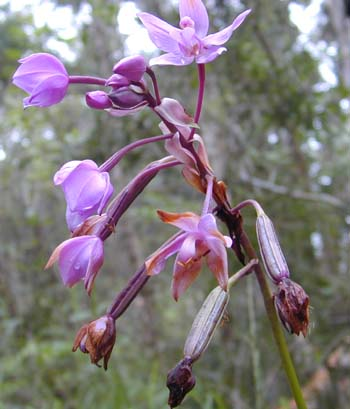
\includegraphics[width=0.7\linewidth]{./figures/plants/Spathoglottis_flwrs_reduced} 

}

\caption{\href{https://commons.wikimedia.org/wiki/File:Spathoglottis_flwrs_reduced.jpg}{Flowers and fruit (capsules) of the ground orchid, Spathoglottis plicata, illustrating an inferior ovary.}}\label{fig:flowersfruits}
\end{figure}

The outer, often edible layer, is the pericarp, formed from the ovary and surrounding the seeds, although in some species other tissues contribute to or form the edible portion. The pericarp may be described in three layers from outer to inner, the epicarp, mesocarp and endocarp.

Fruit that bears a prominent pointed terminal projection is said to be beaked.

A fruit results from maturation of one or more flowers, and the gynoecium of the flower(s) forms all or part of the fruit. Gynoecium (from Ancient Greek γυνή, gyne, meaning woman, and οἶκος, oikos, meaning house) is most commonly used as a collective term for the parts of a flower that produce ovules and ultimately develop into the fruit and seeds. The gynoecium is the innermost whorl of a flower; it consists of (one or more) pistils and is typically surrounded by the pollen-producing reproductive organs, the stamens, collectively called the androecium. The gynoecium is often referred to as the ``female'' portion of the flower, although rather than directly producing female gametes (i.e.~egg cells), the gynoecium produces megaspores, each of which develops into a female gametophyte which then produces egg cells.



\begin{figure}

{\centering 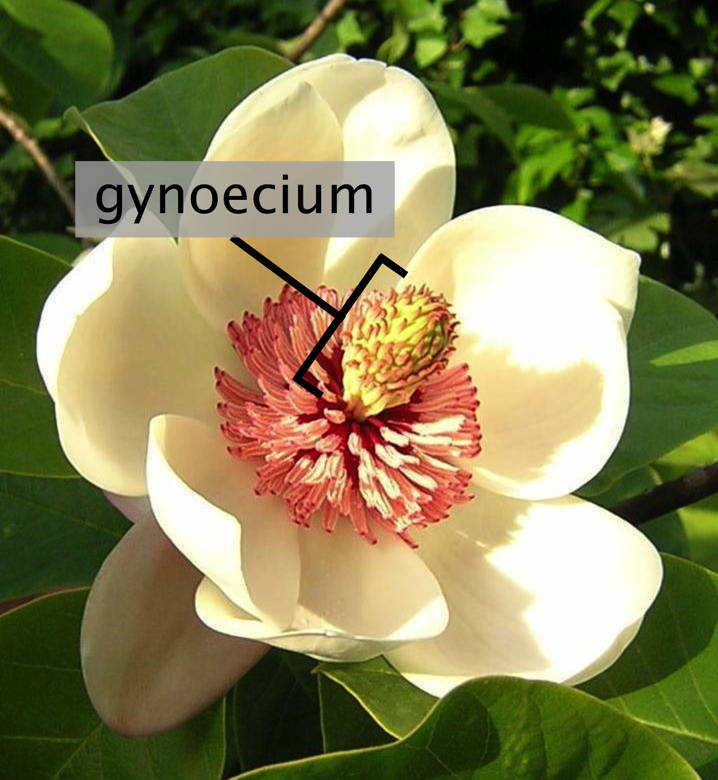
\includegraphics[width=0.7\linewidth]{./figures/plants/Magnolia_wieseneri_-_labelled_gynoecium} 

}

\caption{\href{https://commons.wikimedia.org/wiki/File:Magnolia_wieseneri_-_labelled_gynoecium.jpg}{Flower of Magnolia × wieseneri showing the many pistils making up the gynoecium in the middle of the flower}}\label{fig:gynoecium}
\end{figure}

Inside the ovary/ovaries are one or more ovules where the megagametophyte contains the egg cell. After double fertilization, these ovules will become seeds. The ovules are fertilized in a process that starts with pollination, which involves the movement of pollen from the stamens to the stigma of flowers. After pollination, a tube grows from the pollen through the stigma into the ovary to the ovule and two sperm are transferred from the pollen to the megagametophyte. Within the megagametophyte one of the two sperm unites with the egg, forming a zygote, and the second sperm enters the central cell forming the endosperm mother cell, which completes the double fertilization process. Later the zygote will give rise to the embryo of the seed, and the endosperm mother cell will give rise to endosperm, a nutritive tissue used by the embryo.



\begin{figure}

{\centering 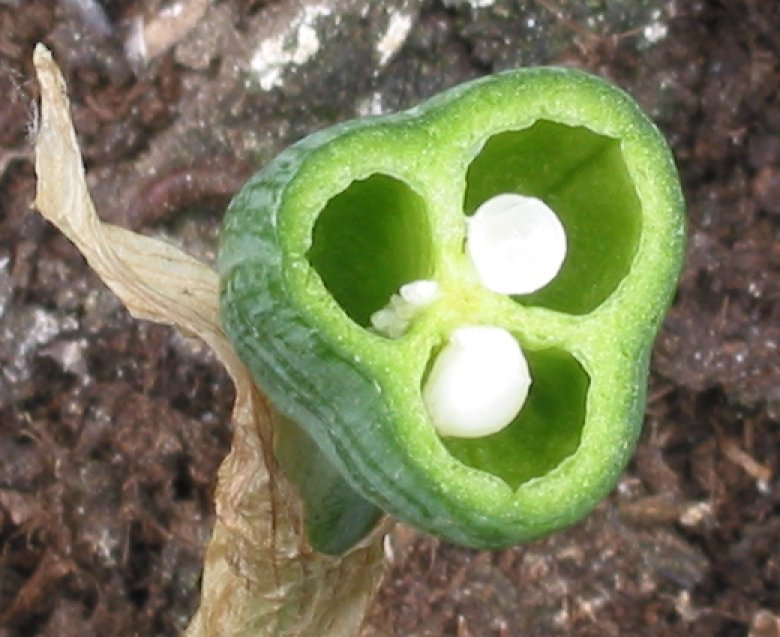
\includegraphics[width=0.7\linewidth]{./figures/plants/Narcis_zaadhokken} 

}

\caption{\href{https://en.wikipedia.org/wiki/Gynoecium\#/media/File:Narcis_zaadhokken.jpg}{Cross-section through the ovary of Narcissus showing multiple carpels (the female reproductive part of the flower) fused along the placental line where the ovules form}}\label{fig:ovarycross}
\end{figure}

As the ovules develop into seeds, the ovary begins to ripen and the ovary wall, the pericarp, may become fleshy (as in berries or drupes), or form a hard outer covering (as in nuts). In some multiseeded fruits, the extent to which the flesh develops is proportional to the number of fertilized ovules. The pericarp is often differentiated into two or three distinct layers called the exocarp (outer layer, also called epicarp), mesocarp (middle layer), and endocarp (inner layer). In some fruits, especially simple fruits derived from an inferior ovary, other parts of the flower (such as the floral tube, including the petals, sepals, and stamens), fuse with the ovary and ripen with it. In other cases, the sepals, petals and/or stamens and style of the flower fall off. When such other floral parts are a significant part of the fruit, it is called an accessory fruit. Since other parts of the flower may contribute to the structure of the fruit, it is important to study flower structure to understand how a particular fruit forms.



\begin{figure}

{\centering 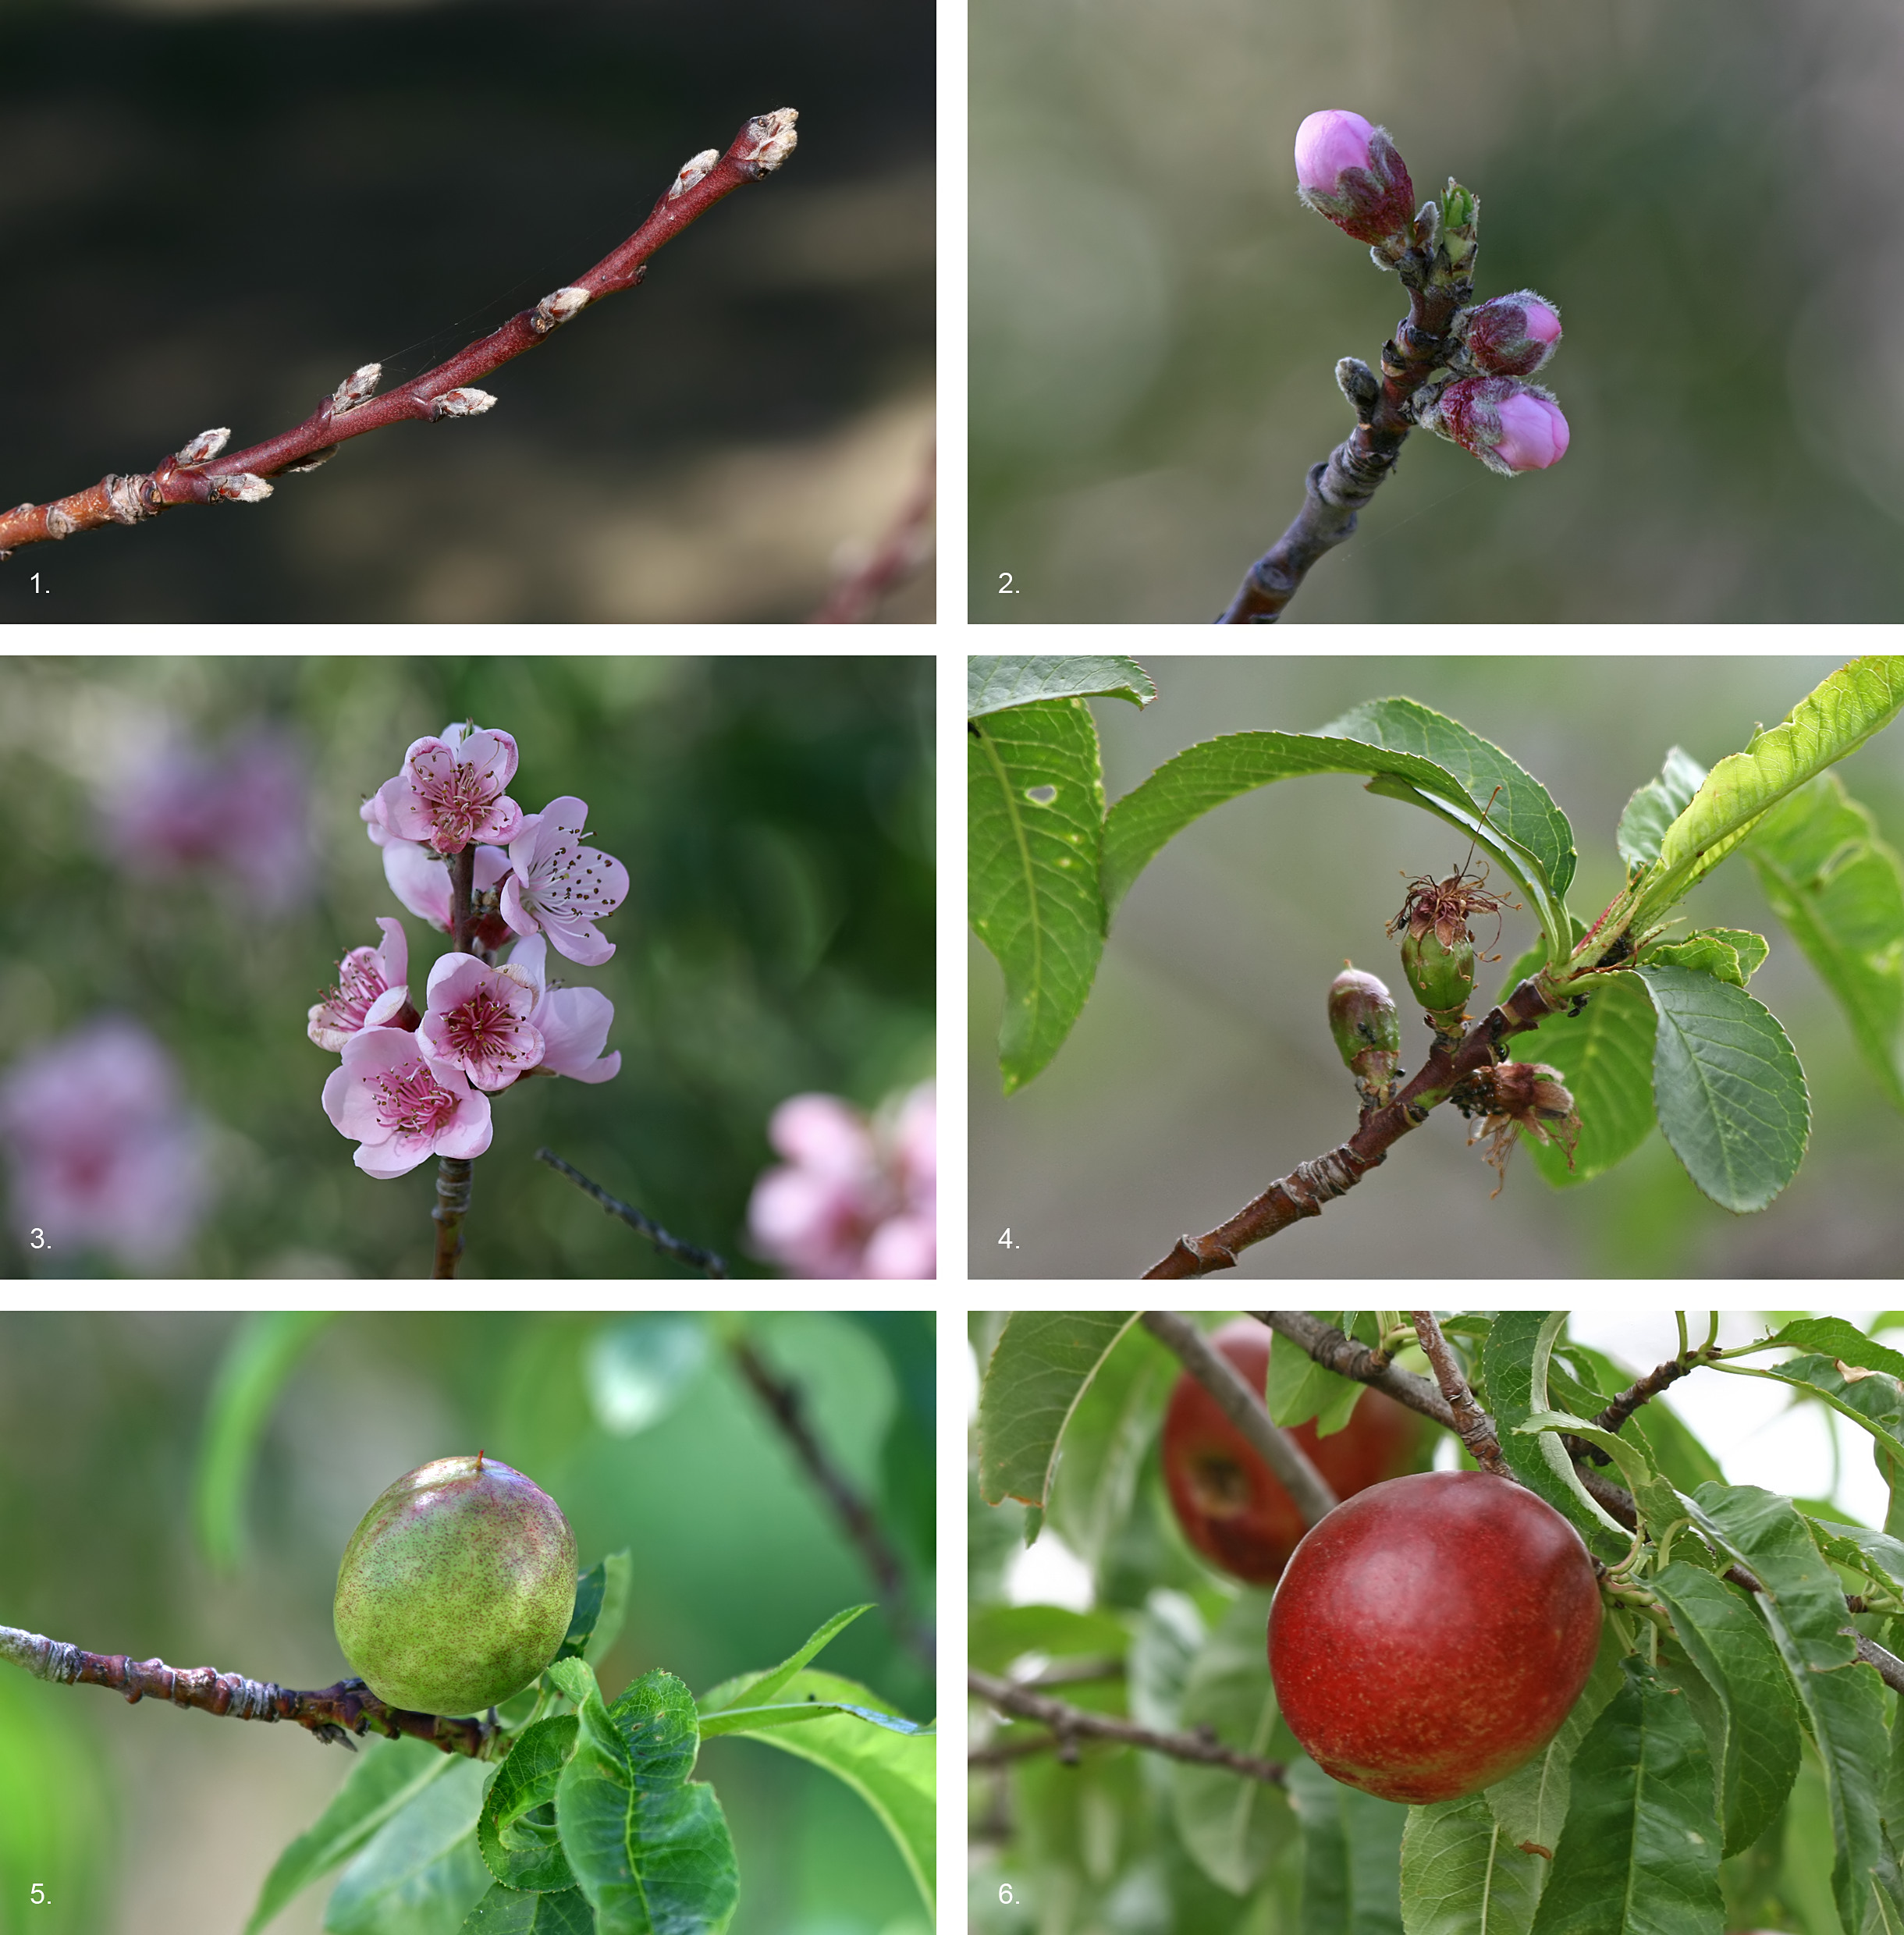
\includegraphics[width=0.7\linewidth]{./figures/plants/Nectarine_Fruit_Development} 

}

\caption{\href{https://commons.wikimedia.org/wiki/File:Nectarine_Fruit_Development.jpg}{The development sequence of a typical drupe, the nectarine (Prunus persica) over a 7.5 month period, from bud formation in early winter to fruit ripening in midsummer.})1. Bud formation can be observed on new growth on the plant (early winter) 2. Flower buds clearly formed and leaves start to develop (early spring, ≈ 3 months) . 3. Flowers fully develop and are pollinated by wind or insects (early spring, ≈ 3½ months). 4. If successfully pollinated, flowers die back and incipient fruit can be observed; leaves have quickly grown to provide tree with food and energy from photosynthesis (mid-spring, ≈ 4 months). 5. Fruit is well developed and continues to grow (late spring, ≈ 5½ months). 6. Fruit fully ripens to an edible form to encourage spreading of seed contained within by animals (midsummer, ≈ 7½ months)}\label{fig:fruitdevelopment}
\end{figure}

There are three general modes of fruit development:

\begin{itemize}
\tightlist
\item
  Apocarpous fruits develop from a single flower having one or more separate carpels, and they are the simplest fruits.
\item
  Syncarpous fruits develop from a single gynoecium having two or more carpels fused together.
\item
  Multiple fruits form from many different flowers.
\end{itemize}

Plant scientists have grouped fruits into three main groups, simple fruits, aggregate fruits, and composite or multiple fruits. The groupings are not evolutionarily relevant, since many diverse plant taxa may be in the same group, but reflect how the flower organs are arranged and how the fruits develop.

\hypertarget{reproductin-of-ferns}{%
\subsection{Reproductin of Ferns}\label{reproductin-of-ferns}}

Ferns are vascular plants differing from lycophytes by having true leaves (megaphylls), which are often pinnate. They differ from seed plants (gymnosperms and angiosperms) in reproducing by means of spores and they lack flowers and seeds. Like all land plants, they have a life cycle referred to as alternation of generations, characterized by alternating diploid sporophytic and haploid gametophytic phases. The diploid sporophyte has 2n paired chromosomes, where n varies from species to species. The haploid gametophyte has n unpaired chromosomes, i.e.~half the number of the sporophyte. The gametophyte of ferns is a free-living organism, whereas the gametophyte of the gymnosperms and angiosperms is dependent on the sporophyte.

The life cycle of a typical fern proceeds as follows:

\begin{enumerate}
\def\labelenumi{\arabic{enumi}.}
\tightlist
\item
  A diploid sporophyte phase produces haploid spores by meiosis (a process of cell division which reduces the number of chromosomes by a half).
\item
  A spore grows into a free-living haploid gametophyte by mitosis (a process of cell division which maintains the number of chromosomes). The gametophyte typically consists of a photosynthetic prothallus.
\item
  The gametophyte produces gametes (often both sperm and eggs on the same prothallus) by mitosis.
\item
  A mobile, flagellate sperm fertilizes an egg that remains attached to the prothallus.
\item
  The fertilized egg is now a diploid zygote and grows by mitosis into a diploid sporophyte (the typical fern plant).
\end{enumerate}

Ferns typically produce large diploids with stem, roots, and leaves; and on fertile leaves called sporangium, spores are produced. The spores are released and germinate to produce short, thin gametophytes that are typically heart-shaped, small and green in color. The gametophytes or thallus, produce both motile sperm in the antheridia and egg cells in separate archegonia. After rains or when dew deposits a film of water, the motile sperm are splashed away from the antheridia, which are normally produced on the top side of the thallus, and swim in the film of water to the antheridia where they fertilize the egg. To promote out crossing or cross-fertilization the sperm is released before the eggs are receptive of the sperm, making it more likely that the sperm will fertilize the eggs of the different thallus. A zygote is formed after fertilization, which grows into a new sporophytic plant. The condition of having separate sporophyte and gametophyte plants is called alternation of the generations. Other plants with similar reproductive means include the Psilotum, Lycopodium, Selaginella and Equisetum.

\hypertarget{reproductin-of-bryophytes}{%
\subsection{Reproductin of Bryophytes}\label{reproductin-of-bryophytes}}

The bryophytes, which include liverworts, hornworts and mosses, reproduce both sexually and vegetatively. The gametophyte is the most commonly known phase of the plant. All are small plants found growing in moist locations and like ferns, have motile sperm with flagella and need water to facilitate sexual reproduction. These plants start as a haploid spore that grows into the dominant form, which is a multicellular haploid body with leaf-like structures that photosynthesize. Haploid gametes are produced in antheridia and archegonia by mitosis. The sperm released from the antheridia respond to chemicals released by ripe archegonia and swim to them in a film of water and fertilize the egg cells, thus producing zygotes that are diploid. The zygote divides by mitotic division and grows into a sporophyte that is diploid. The multicellular diploid sporophyte produces structures called spore capsules. The spore capsules produce spores by meiosis, and when ripe, the capsules burst open and the spores are released. Bryophytes show considerable variation in their breeding structures and the above is a basic outline. In some species each gametophyte is one sex while other species produce both antheridia and archegonia on the same gametophyte which is thus hermaphrodite.


